A case study of a fabricated measles outbreak is discussed in \S \ref{sec:res_caseS}, which is used for the generation of the results in this chapter. The base set of parameters used is discussed in \S \ref{sec:res_baseCase}, along with a presentation of the base case of the epidemic model using those parameters. Results regarding the resource allocation models and delivery methods tested are discussed in \S \ref{sec:res_resAllocModel} and \S \ref{sec:res_delMethRes}, respectively. Sensitivity analysis is performed on the parameters outside of the control of intervention decision-makers, in \S \ref{sec:res_sensAn}. The chapter is concluded with an evaluation of scenario tests and factors which are under the control of intervention decision-makers, in \S \ref{sec:res_scenTests}.

\section{Case study}
\label{sec:res_caseS}
In order to obtain results, compare resource allocation strategies and evaluate UAV delivery as an alternative to vehicle vaccine delivery, a fabricated measles outbreak is simulated in Likasi and surrounds, in the Democratic Republic of Congo (DRC). Likasi is a large city of over 400\,000 people, with a number of smaller towns and villages nearby -- some of which are only accessible by unmarked paths and roads, which are likely impassable at times. In this case, the number of locations is $n = 12.$ A map of the area is illustrated in Figure \ref{map:likasi}.

\begin{figure}[ht!]{\textwidth}
    \centering
    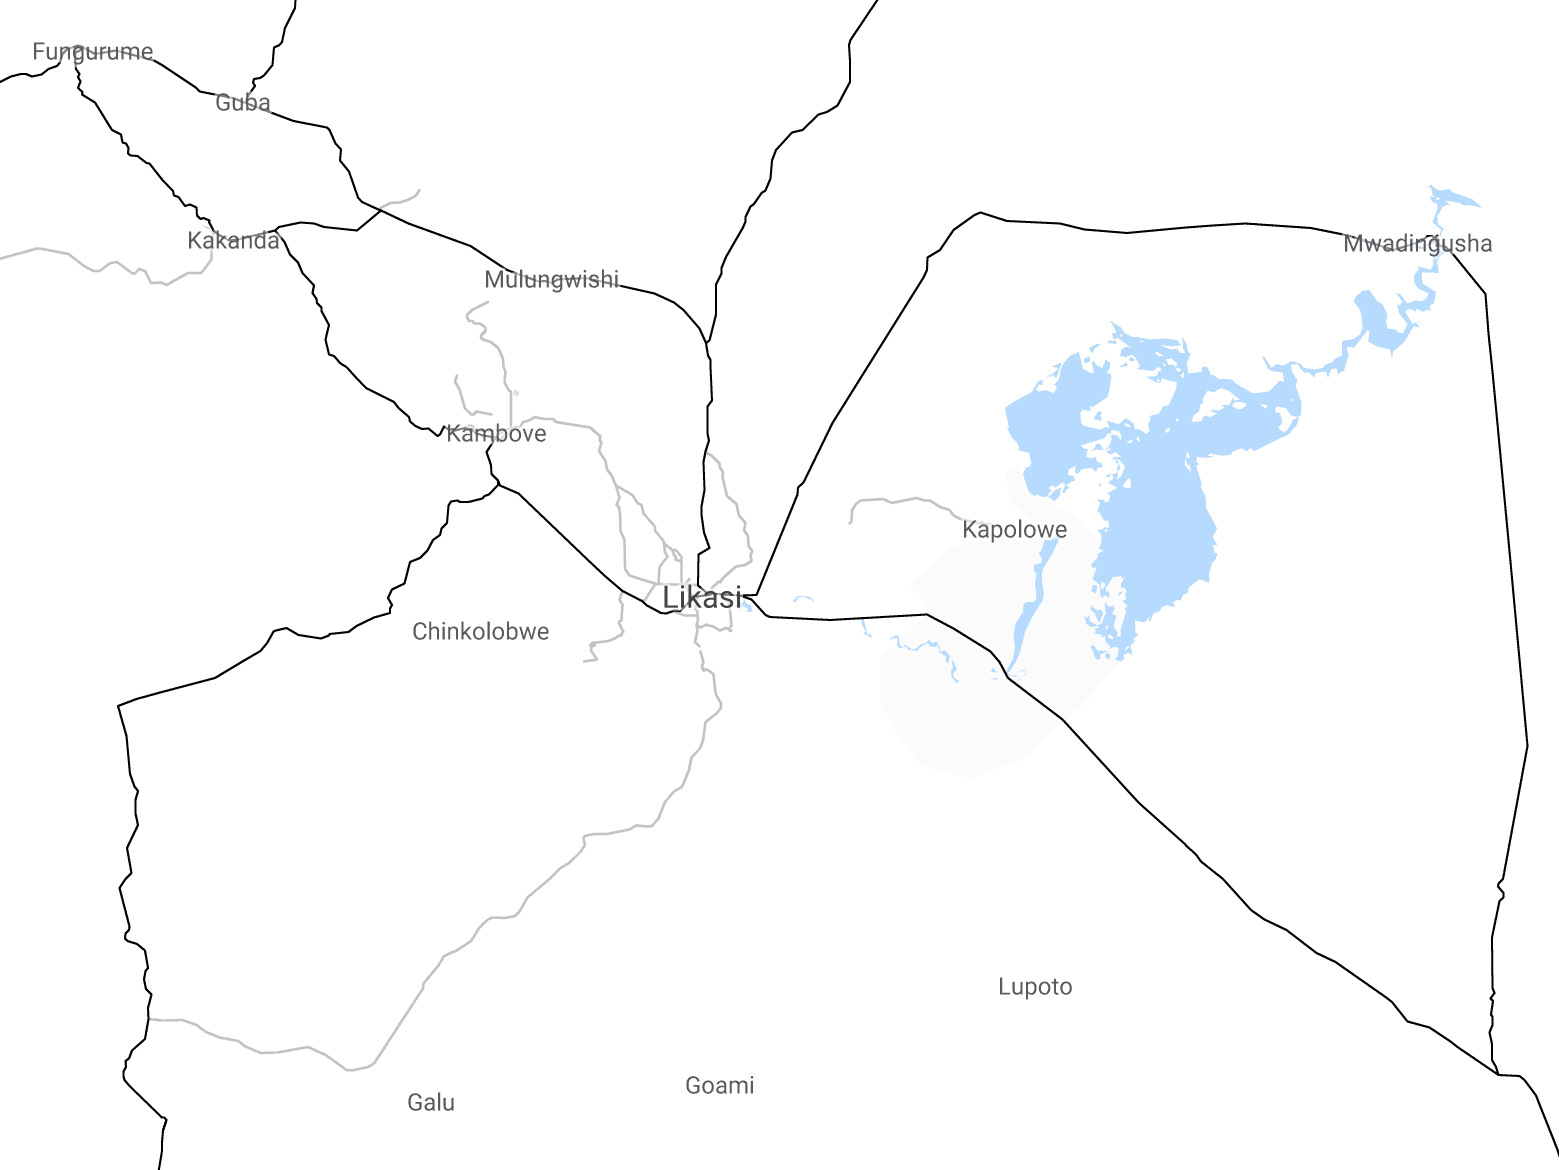
\includegraphics[width=0.8\textwidth]{likasi.png}
    \caption{Map of Likasi and surrounds, Democratic Republic of Congo}
    \label{map:likasi}
\end{figure}

Road distances between locations were procured from Google Maps, and Cartesian coordinates of the locations were estimated. Table \ref{tab:roadDistances} contains the road distances found. If there is no direct road between locations $i$ and $j$, the distance is marked as unavailable. If there is a direct road, the distance is given in kilometres.

\begin{table}[h]
\centering
\resizebox{\textwidth}{!}{%
\begin{tabular}{|c|cccccccccccc|}
\hline
 & \multicolumn{1}{c|}{Fungurume} & \multicolumn{1}{c|}{Guba} & \multicolumn{1}{c|}{Kakanda} & \multicolumn{1}{c|}{Mul...shi} & \multicolumn{1}{c|}{Kambove} & \multicolumn{1}{c|}{Chi...bwe} & \multicolumn{1}{c|}{Likasi} & \multicolumn{1}{c|}{Kapolowe} & \multicolumn{1}{c|}{Mwa...sha} & \multicolumn{1}{c|}{Galu} & \multicolumn{1}{c|}{Goami} & Lupoto \\ \hline
Fungurume & 0 & 12 & 24 & - & - & - & - & - & - & - & - & - \\ \cline{1-1}
Guba & 12 & 0 & 27 & 28 & - & - & - & - & - & - & - & - \\ \cline{1-1}
Kakanda & 24 & 27 & 0 & 25 & 29 & - & - & - & - & - & - & - \\ \cline{1-1}
Mulungwishi & - & 28 & 25 & 0 & - & - & 34 & - & - & - & - & - \\ \cline{1-1}
Kambove & - & - & - & 29 & 0 & - & 25 & - & - & - & - & - \\ \cline{1-1}
Chinkolobwe & - & - & - & - & - & 0 & - & - & - & - & - & - \\ \cline{1-1}
Likasi & - & - & - & 34 & 25 & - & 0 & 32 & 73 & 50 & - & - \\ \cline{1-1}
Kapolowe & - & - & - & - & - & - & 32 & 0 & 70 & - & - & - \\ \cline{1-1}
Mwandingusha & - & - & - & - & - & - & 73 & 70 & 0 & - & - & - \\ \cline{1-1}
Galu & - & - & - & - & - & - & 50 & - & - & 0 & - & - \\ \cline{1-1}
Goami & - & - & - & - & - & - & - & - & - & - & 0 & - \\ \cline{1-1}
Lupoto & - & - & - & - & - & - & - & - & - & - & - & 0 \\ \hline
\end{tabular}
}
\caption{Distances by road between locations in the network (in kilometres).}
\label{tab:roadDistances}
\end{table}

The population values used are contained in Table \ref{tab:podDetails}, split into categories for vaccinated (V) and susceptible (S), as well as exposed (E), infected (I) and recovered (R). Scaled euclidean coordinates of the locations (x,y) are included in Table \ref{tab:podDetails}, as well as a column indicating whether the location is urban or not.  In the table, the columns \textit{mapX} and \textit{mapY} represent (x,y) coordinates for plotting the location's details on the map, and are not used for calculations. Note that all previously-vaccinated individuals are placed in the V category and thus, vaccination is targeted to individuals with no history of previous vaccination. 

\begin{table}[h]
\centering
\resizebox{\textwidth}{!}{%
\begin{tabular}{|c|ccccccccccc|}
\hline
 & \multicolumn{1}{c|}{Urban} & \multicolumn{1}{c|}{x} & \multicolumn{1}{c|}{y} & \multicolumn{1}{c|}{N} & \multicolumn{1}{c|}{S} & \multicolumn{1}{c|}{E} & \multicolumn{1}{c|}{I} & \multicolumn{1}{c|}{R} & \multicolumn{1}{c|}{V} & \multicolumn{1}{c|}{mapX} & \multicolumn{1}{c|}{mapY} \\ \hline
Fungurume & 1 & 7.11 & 105.69 & 18400 & 5152 & 0 & 0 & 0 & 13258 & 87 & 35 \\ \cline{1-1}
Guba & 1 & 17.83 & 100.03 & 920 & 258 & 0 & 0 & 0 & 662 & 243 & 87 \\ \cline{1-1}
Kakanda & 1 & 16.54 & 88.54 & 9200 & 2576 & 0 & 0 & 0 & 6624 & 225 & 227 \\ \cline{1-1}
Mulungwishi & 1 & 39.43 & 86.83 & 4600 & 1288 & 0 & 0 & 0 & 3312 & 541 & 265 \\ \cline{1-1}
Kambove & 1 & 36.60 & 75.86 & 17020 & 4766 & 0 & 0 & 0 & 12254 & 483 & 415 \\ \cline{1-1}
Chinkolobwe & 0 & 33.69 & 62.14 & 184 & 52 & 0 & 0 & 0 & 132 & 469 & 611 \\ \cline{1-1}
Likasi & 1 & 48.60 & 64.71 & 207000 & 57960 & 0 & 5 & 0 & 149035 & 703 & 579 \\ \cline{1-1}
Kapolowe & 1 & 72.69 & 69.17 & 6440 & 1803 & 0 & 0 & 0 & 4637 & 1007 & 515 \\ \cline{1-1}
Mwandingusha & 0 & 106.46 & 90.00 & 1840 & 515 & 0 & 0 & 0 & 1325 & 1413 & 231 \\ \cline{1-1}
Galu & 0 & 33.60 & 26.40 & 276 & 77 & 0 & 0 & 0 & 199 & 433 & 1081 \\ \cline{1-1}
Goami & 0 & 53.74 & 27.86 & 120 & 34 & 0 & 0 & 0 & 86 & 715 & 1065 \\ \cline{1-1}
Lupoto & 0 & 75.00 & 36.43 & 230 & 64 & 0 & 0 & 0 & 156 & 1031 & 961 \\ \hline
\end{tabular}%
}
\caption{Network location details, including populations and coordinates.}
\label{tab:podDetails}
\end{table}

Population values for the network locations were estimated using census data, and satellite imagery when data was unavailable. Measles vaccinations are usually performed on children aged 9 months to 15 years, as early as possible \cite{danet_fermon_2013}. Since 46\% of the population in the DRC are below the age of 15 \cite{demographic_dividend}, and the measles vaccination rate in the country is most recently estimated to be 72\% \cite{who_2018_coverage}, the number of susceptible people used as input for the model is significantly less than the total population.

\section{Epidemic model results}
\label{sec:res_baseCase}
Since the simulation has many components which vary randomly , repeated simulations are required to nullify any random biases in the results. This repeated simulation is performed according to the process described in \S \ref{sec:meth_sim_res}, with a base set of initial parameter values listed in Table \ref{tab:res_baseParams}.

\begin{table}[ht!]
\centering
\resizebox{\textwidth}{!}{%
\begin{tabular}{|c|c||c|c|}
\hline
\multicolumn{1}{|c|}{\textbf{Parameter}} & \textbf{Value} & \multicolumn{1}{c|}{\textbf{Parameter}} & \textbf{Value}  \\ \hline
$\sigma$                         & $\frac{1}{10}$ &    Death Rate                       & 10\%              \\
$\beta$                          & $\frac{15}{8}$ & Work days per week                & 7 days               \\
$\gamma$                    & $\frac{1}{8}$       & Intervention delay      & 15 days         \\
$R_{0}$                         & 15            & Intervention length                     & 28 days \\
$k_{m}$                          & 1              & Primary vehicle capacity         & 1050 vaccines   \\
$\mu$                       & $\frac{0.1}{8}$   & Secondary vehicle capacity      & 200 vaccines        \\
$\lambda_{S}$                  & 0.95           & UAV capacity                    & 60 vaccines      \\
$\lambda_{E}$                   & 0.83           & Average UAV speed               & 100 km/h        \\
$\mathcal{K}$                   & 1             & Combined delivery cutoff time   & 180 minutes   \\
$\mathcal{N}$                   & 15 teams      &  $\psi_{i}$ per fixed-post team  & 450 vaccinations \\   
$\mathcal{H}$                 & 660 minutes    & $\psi_{i}$ per mobile team   & 250 vaccinations     \\
Epidemic detection ratio     & 0.5\%           & Number of vehicles   &  2   \\ \hline
\end{tabular}%
}
\caption{Base set of parameters for simulation.}
\label{tab:res_baseParams}
\end{table}

A base case of the simulation is performed with no vaccine deliveries and epidemic parameters set to the values given in Table \ref{tab:res_baseParams}. 
The progression of the population between the different compartmental model categories is shown in Figure \ref{fig:SEIRnoV}. Most of the population becomes infected with measles and recovers, although there are a significant number of deaths also. Repeating this simulation 500 times gives an average of 6\,504 deaths per epidemic. 

\begin{figure}[ht]{\textwidth}
    \centering
     \subfloat[Epidemic progression without intervention.]{
       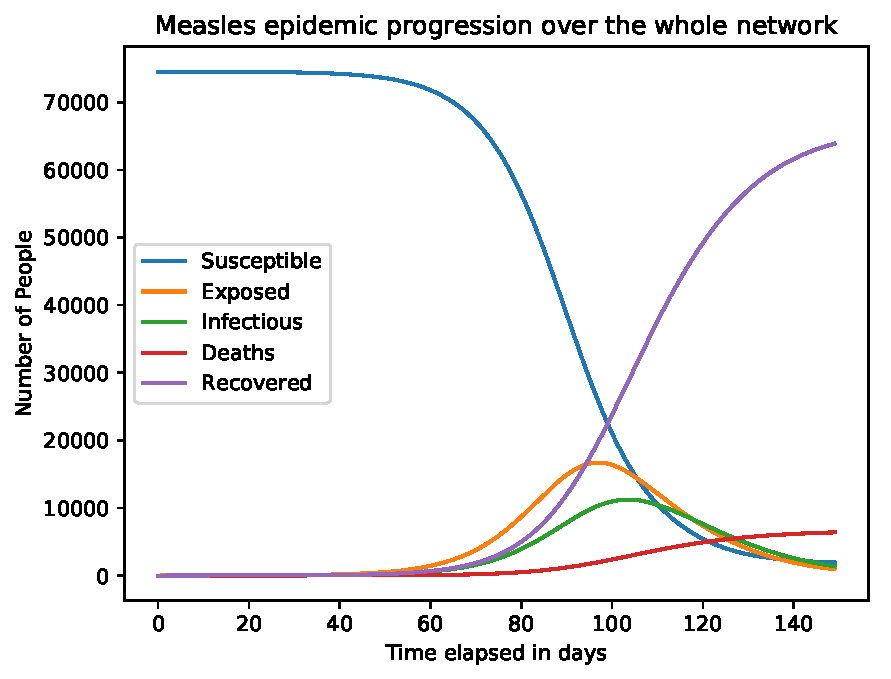
\includegraphics[width=0.48\textwidth, trim={0 0 0 0.7cm}, clip]{Figures/SEIRnoV.pdf}
       \label{fig:SEIRnoV}
     }
     \subfloat[Epidemic progression with intervention.]{
       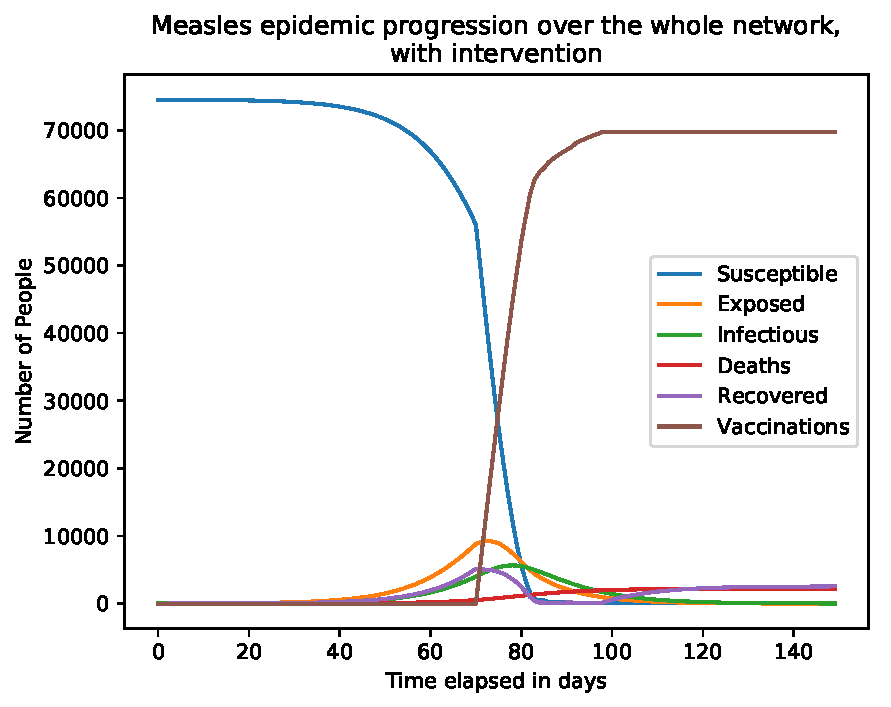
\includegraphics[width=0.48\textwidth, trim={0 0 0 1.2cm}, clip]{Figures/SEIRvehicleD.pdf}
       \label{fig:SEIRvehicleD}
     }
     %add epidemic progression with constant vaccinations intervention
    \caption{Progression of simulated measles epidemic with and without intervention.}
\end{figure}

In Figure \ref{fig:SEIRvehicleD}, the progression of the population between categories, where there is vaccination according to the set of base parameters in Table \ref{tab:res_baseParams}, is shown. Vehicle delivery was used with vaccine allocation strategy $I$ and team allocation strategy $N$. Clearly, vaccination curbs the epidemic's progress considerably -- resulting in an average number of just 2\,212 deaths, at an average total delivery and vaccine cost of \$362\,523.

\section{Resource allocation model results}
\label{sec:res_resAllocModel}
As discussed in detail in \S \ref{sec:vd_strat} and \S \ref{sec:team_strat} respectively, different strategies for vaccine deliveries and team allocations can be employed for an intervention. The team assignment strategies include assigning teams proportionally to I, S, N, or I/N, or to assign them equally across the network, with each location having at least one team. The optimal EPE team assignment strategy can also be used. 

The vaccine delivery strategy determines which locations receive vaccines first, and can be one of I, S, or N, or the optimised EPE delivery strategy. To test which pair of team and vaccine delivery strategies is best, each pair was simulated 500 times, to produce the average results plotted in Figure \ref{fig:res_teamScatter}, and recorded in more detail in Table \ref{tab:vehicle_stratPairs} in Appendix A. For each of the six team strategies, each of the four delivery strategies is simulated and plotted as a point in Figure \ref{fig:res_teamScatter}. The delivery strategy is represented with a letter, and the team strategy by different colours -- so each point is the result of 500 simulations with that strategy pair. As is clear in the figure from the distinct clusters, results are much more dependant upon the team strategy than the delivery strategy. The choice of delivery strategy has very little bearing on the cost or number of deaths, so any delivery strategy used will be successful if the teams are well allocated.

\begin{figure}[ht!]
    \centering
    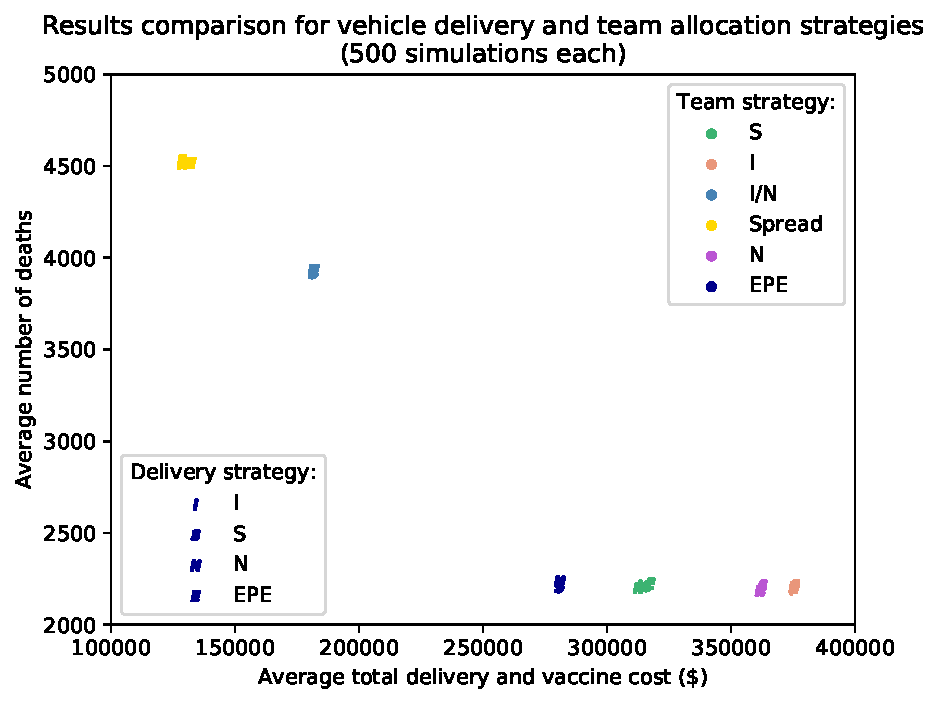
\includegraphics[width=0.9\textwidth, trim={0 0 0 1.15cm}, clip]{teamAssScatter.pdf}
    \caption{Comparison of various vaccine delivery and team assignment strategy pairs, with vehicle delivery for vaccines.}
    \label{fig:res_teamScatter}
\end{figure}

Take note of the four bottom-right clusters in Figure \ref{fig:res_teamScatter}. These four team-allocation strategies (EPE, S, N and I) are clearly the best strategies for minimising deaths, although they incur a higher average total cost. This higher cost is primarily due to a higher number of vaccines administered, causing the reduction in deaths. The strategy pair with the lowest average deaths is (N,N); 2184 deaths at a cost of \$361\,751. The EPE team allocation strategy, paired with the S vaccine delivery strategy, results in an average of 2204 deaths at a cost of \$280\,735. This is a \$35\,196 cost saving from the next cheapest intervention with a similar level of deaths, and a similar number of lives saved to the (N,N) strategy, for a cost of \$81\,016 (22.4\%) less. The EPE team allocation strategy significantly reduces average total delivery and vaccine cost when compared to other strategies with similar numbers of deaths.

For a visual representation of the difference between resource allocation strategy pairs, a selection of pairs were each simulated 500 times, producing the plot shown in Figure \ref{fig:res_avgVaccsPerDay}. This, for each team allocation strategy paired with an appropriate vaccine delivery allocation strategy, shows the average number of vaccinations per day during the simulation. On average, interventions begin between day 60 and 80, and end before day 110. The four best team allocation strategies discussed earlier (EPE, S, N, and I) vaccinate the most people, with the other two strategies performing poorly and not vaccinating enough people to prevent deaths. The cost improvement found for the EPE and S team allocation strategies clearly occurs towards the end of the intervention; while the I and N strategies continue vaccinations, the EPE and S strategies stop. Towards the end of the epidemic, as can be seen in Figure \ref{fig:SEIRvehicleD}, there are essentially no susceptible individuals remaining. Therefore, the I and N strategies waste vaccines on already-recovered and exposed individuals, where those vaccinations actually have no impact. 

The effect of the different resource allocation strategies on a medium-sized town is shown in Figure \ref{fig:res_avpdFungurume}, where the average number of daily vaccinations over time is plotted for each of six strategy pairs, in the town of Fungurume (with population 18\,400). Initially, the epidemic has not yet spread to Fungurume, and only the S, N, and spread strategies perform vaccinations. When the epidemic spreads to Fungurume, there is a large spike in vaccinations for the EPE strategy; since there is now potential for many exposures in Fungurume, many vaccinations are performed. The I and I/N strategies result in vaccinations being performed towards the end of the intervention, only once there are a significant number of infections in Fungurume. 

Clearly, intervention should end once it seems clear that all susceptible people have been vaccinated, in order to reduce cost. This is implemented by the EPE and S strategies well, and therefore they should generally be good strategies for resource allocation decisions.

\begin{figure}[ht!]{\textwidth}
    \centering
     \subfloat[Average number of daily vaccinations over time, for a range of resource allocation strategy pairs (team strategy, followed by delivery strategy).]{
       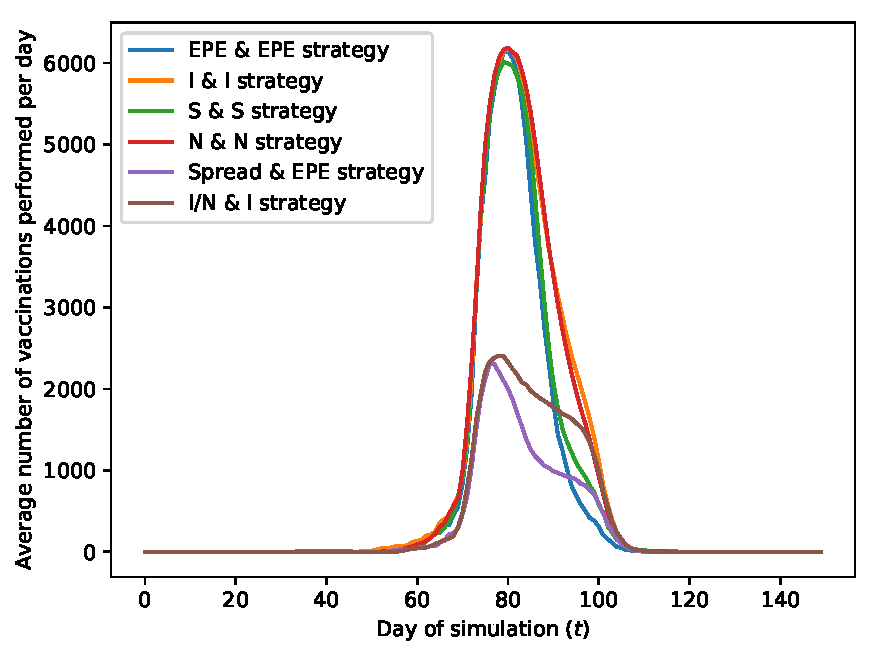
\includegraphics[width=0.47\textwidth]{Figures/vaccCompPlot.pdf}
       \label{fig:res_avgVaccsPerDay}
     }
     \vspace{4}
     \subfloat[Average daily vaccinations over time in Fungurume, for a range of resource allocation strategy pairs.]{
       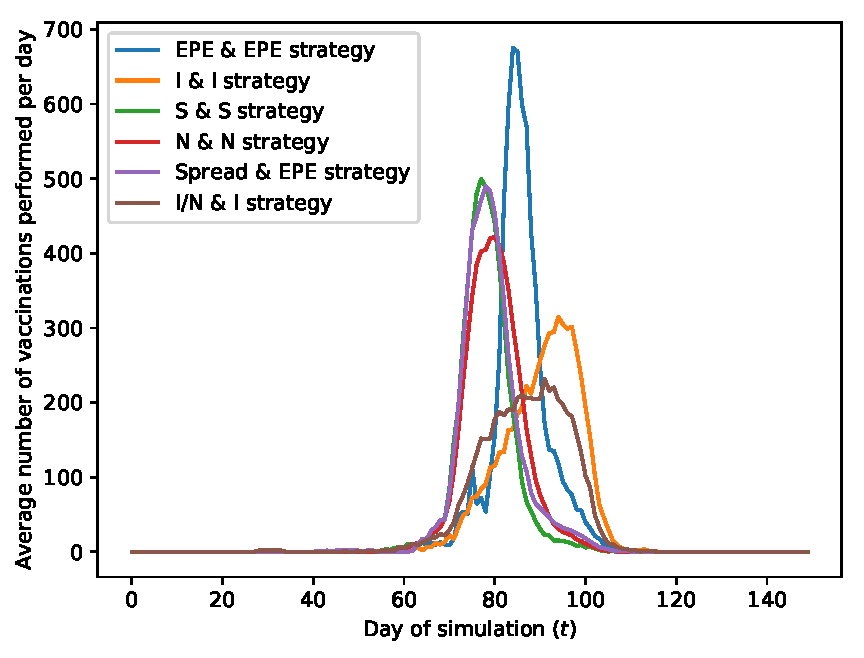
\includegraphics[width=0.47\textwidth]{Figures/vaccCompPlotFungurume.pdf}
       \label{fig:res_avpdFungurume}
     }
    \caption{Depiction of resource allocation strategies over time.}
    \end{figure}

The selection of which locations receive priority for vaccinations also poses an ethical dilemma of sorts. Rural locations generally have worse health infrastructure and consequently, a higher likelihood of measles resulting in death, but urban locations have higher transmission rates. Whether it is best to minimise deaths and exposures across an entire network, or only in cities or rural areas, is a question that cannot necessarily be answered by quantitative methods. To that end, further investigation into resource allocation strategies based on fairness and equity is an interesting topic for future work.

\section{Delivery method results}
\label{sec:res_delMethRes}
A central focus of this project is evaluating the possibility of a UAV delivery network in comparison to a vehicle-based network, or perhaps as an addition to it. Initially, there is assumed to be 2 vehicles available for the vehicle-only network, 2 UAVs for the UAV-only network, and one of each for the combined network. In the combined network, UAVs are used for vehicle deliveries that would take longer than 3 hours.

These three vaccine delivery networks are compared on the basis of cost and deaths, for each pair of team allocation and vaccine delivery strategies. The results of this comparison are plotted in Figure \ref{fig:res_delMethods}, and are listed in more detail in Tables \ref{tab:vehicle_stratPairs}, \ref{tab:UAV_stratPairs}, and \ref{tab:Combined_stratPairs}, of Appendix A.

\begin{figure}[ht!]
    \centering
    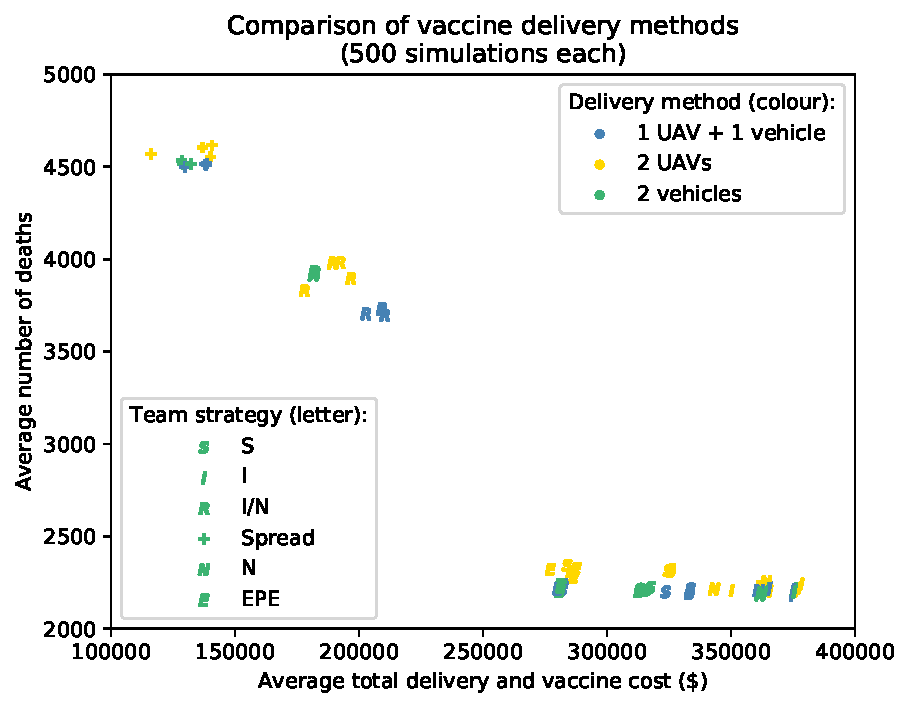
\includegraphics[width=0.9\textwidth, trim={0 0 0 1.15cm}, clip]{Figures/delivMethodScatter.pdf}
    \caption{Comparison of vaccine delivery methods on cost and deaths.}
    \label{fig:res_delMethods}
\end{figure}

Considering Figure \ref{fig:res_delMethods}, the clustering of team strategies is evident as in the vehicle-only network plotted in Figure \ref{fig:res_teamScatter}, although the UAV network's results are more widely spread. All three networks offer similar results to one another, but the UAV network results in marginally more deaths for most strategy pairs. This is due to the small payload of the UAVs, preventing the UAV network from delivering as many vaccines on time as are required. However, having 3 or more UAVs (as shown in Figure \ref{fig:res_numUAVs}) puts the UAV network on par with the vehicle network. 

As can be seen in Figure \ref{fig:res_numVehs}, there is no significant improvement in the delivery network for more than 1 vehicle (because a single vehicle can meet demand for vaccines most of the time). The results of different combinations of vehicles and UAVs are contained in Table \ref{tab:combiSims}, in Appendix A -- they also indicate essentially no change in the delivery network's performance when more vehicles or UAVs are added, for more than 2 UAVs.

\begin{figure}[ht!]{\textwidth}
\centering
 \subfloat[Comparison of number of UAVs on results.]{
   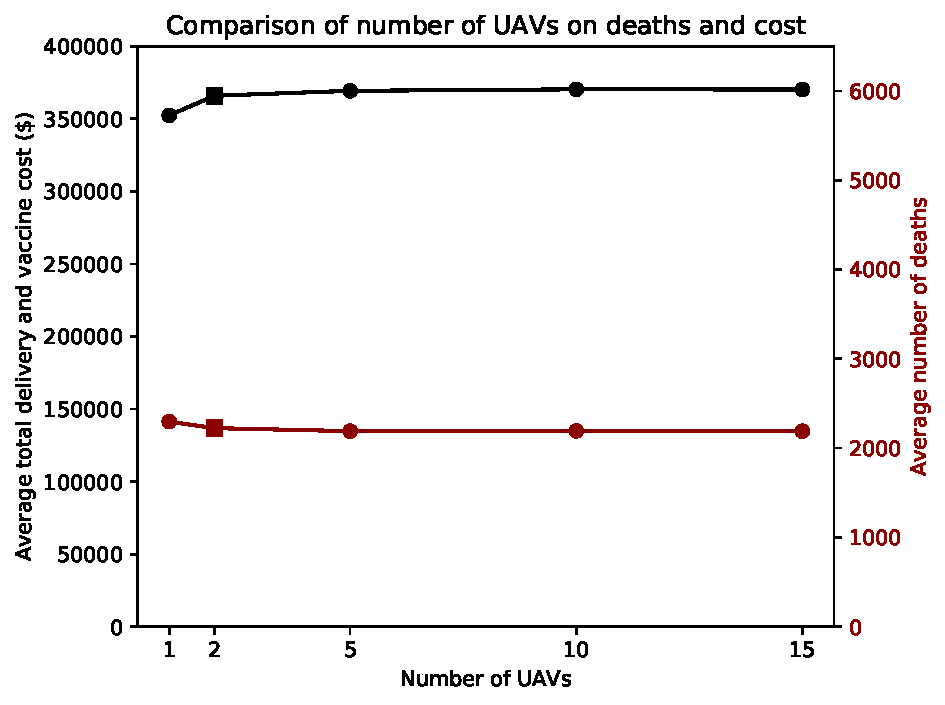
\includegraphics[width=0.48\textwidth, trim={0 0 0 0.67cm}, clip]{Figures/NumberofUAVs.pdf}
   \label{fig:res_numUAVs}
 }
 \subfloat[Comparison of number of vehicles on results.]{
   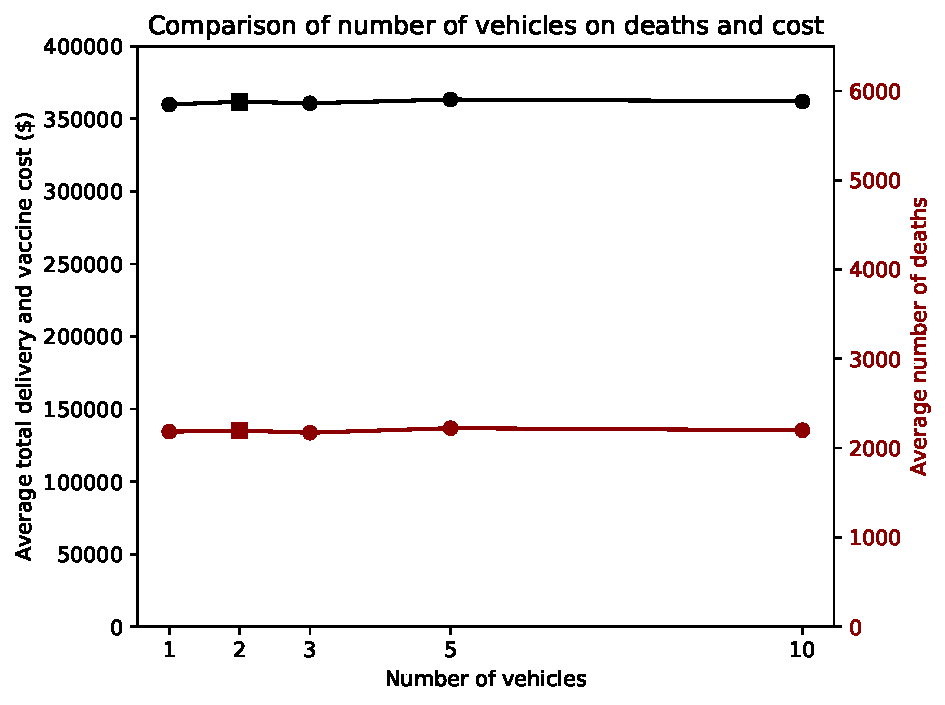
\includegraphics[width=0.48\textwidth, trim={0 0 0 0.67cm}, clip]{Figures/Numberofvehicles.pdf}
   \label{fig:res_numVehs}
 }
\hspace{1pt}
 \subfloat[Effect of differing numbers of impassable roads on results, out of 24 roads in total.]{
   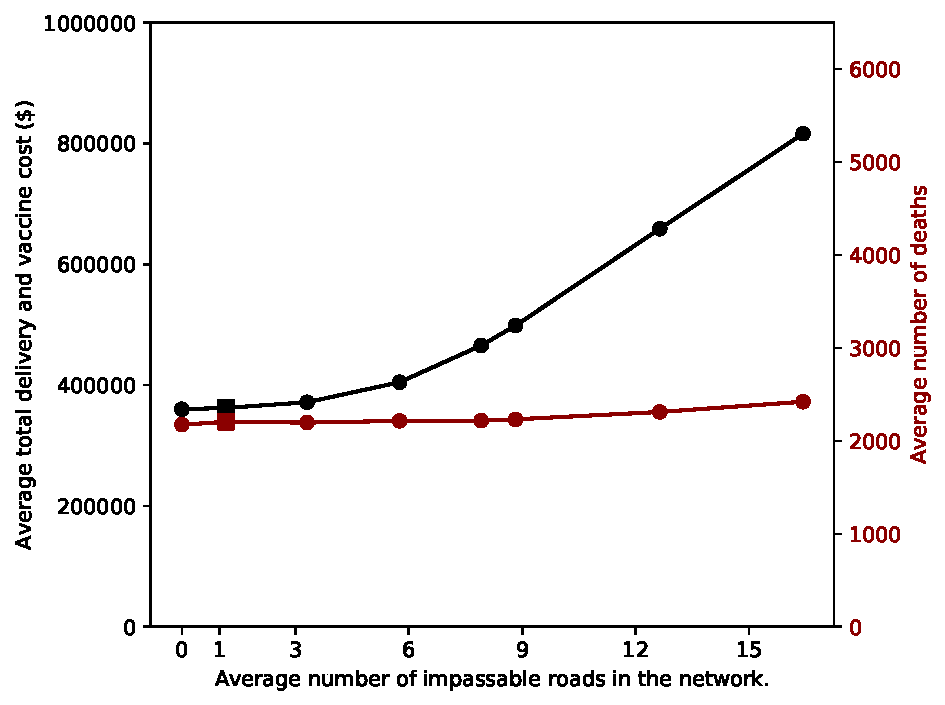
\includegraphics[width=0.48\textwidth]{roads.pdf}
   \label{fig:res_roadProb}
 }

\caption{Effect of differing numbers of UAVs and vehicles, and differing numbers of closed roads, on the performance of vaccine delivery networks.}
\end{figure}

Figure \ref{fig:res_roadProb} shows the impact of worsened road conditions on the average simulated costs and deaths. Clearly, the delivery cost increases exponentially as more roads are set as impassable, while the average number of deaths also rises slightly. This is due to deliveries taking longer, and thus requiring more petrol. With the same resource allocation strategy pair, the average simulated cost of UAV deliveries is \$364\,479 and the average number of deaths is 2\,204. Therefore, if 3 or more roads are closed in the network, UAV delivery (using only 2 UAVs) is cheaper, and results in fewer deaths. Note that there are 24 roads in the network, so this translates to a percentage of 12.5\% of roads; if more than 12.5\% of roads in a network are impassable, UAVs should be a better delivery method than vehicles. However, this is highly dependant on the structure of the network and so, the determination of this `break-even' percentage can be improved by considering a wide range of different networks. This is a good topic for future research; to determine at which point it is better to use UAVs than vehicles, based on a variety of network structures.

As is clear in Figures \ref{fig:res_numUAVs} and \ref{fig:res_roadProb}, UAV delivery with 3 or more UAVs is on par with vehicle delivery networks -- even those on perfect road networks. It can thus be concluded that in locations with poor road infrastructure, UAV delivery is cheaper and more effective than land-based delivery at reducing deaths.

\section{Sensitivity Analysis}
\label{sec:res_sensAn}
Parameters which are mostly out of the control of intervention decision-makers are discussed in this section, to evaluate which parameters have a large impact on average costs and deaths, the output parameters of the simulation.
The approach followed for testing the model output for sensitivity to parameters is varying each parameter individually from its base value, with all other parameters held constant. As each parameter is increased and decreased, changes to the model output parameters (costs and deaths) are observed. The changes in each parameter are according to a range of reasonable values for that parameter. This approach is among those discussed by Pannell \cite{pannell1997sensitivity} for sensitivity analysis. Unless otherwise stated, vehicle deliveries with vaccine allocation strategy $I$ and team allocation strategy $N$ were used in the sensitivity analysis.

\subsubsection{Measles epidemic model parameters}
There are five significant parameters governing the spread of the simulated measles epidemic between individuals, and across locations. The values $\beta, \sigma, \gamma \text{ and } \mu$ determine the movement of individuals between the S and E, E and I, I and R, and I and D classes, respectively. Finally, the fifth parameter $k_{m}$ is a migration frequency multiplier, used in the migration model discussed in \S \ref{sec:meth_migration}. The amount of migration between locations in the model is directly proportional to the value of $k_{m}$, which, in turn, directly affects the speed at which the epidemic spreads between locations.

\begin{figure}[ht!]{\textwidth}
    \centering
     \subfloat[Comparison of durations of exposure.]{
       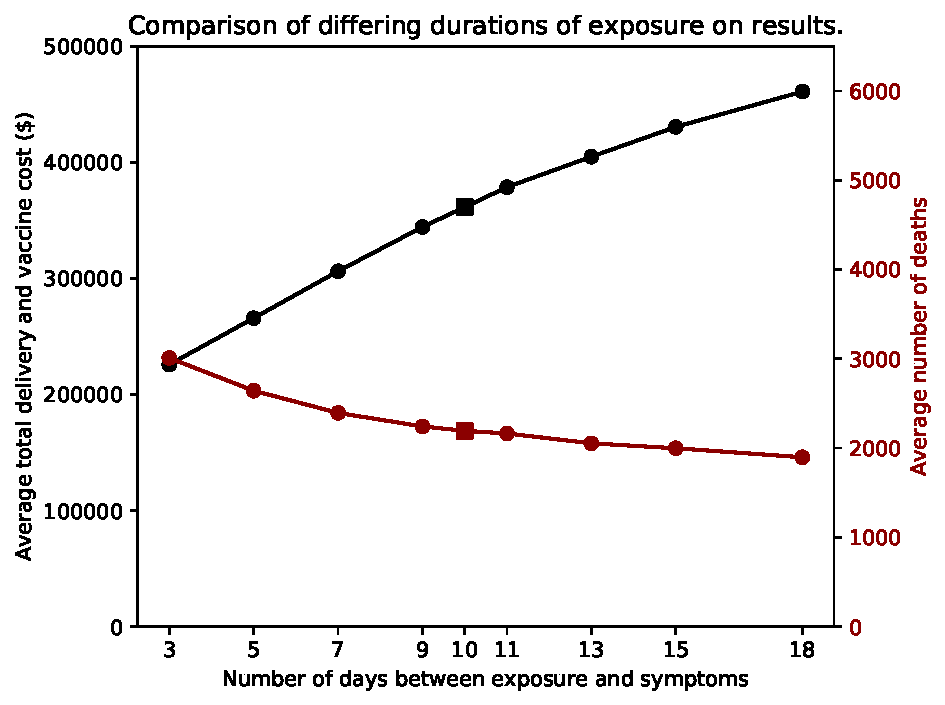
\includegraphics[width=0.48\textwidth, trim={0 0 0 0.67cm}, clip]{Figures/expDays.pdf}
       \label{fig:expDays}
     }
     \subfloat[Comparison of durations of infection.]{
       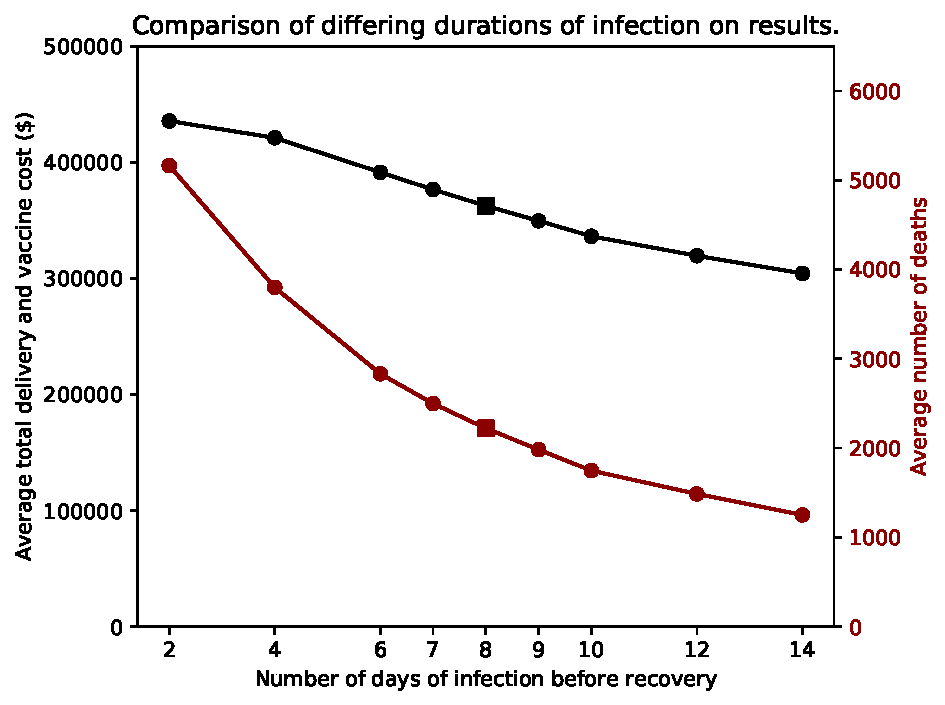
\includegraphics[width=0.48\textwidth, trim={0 0 0 0.67cm}, clip]{Figures/infDays.pdf}
       \label{fig:infDays}
     }
     \vspace{2pt}
     \subfloat[Comparison of death rates.]{
       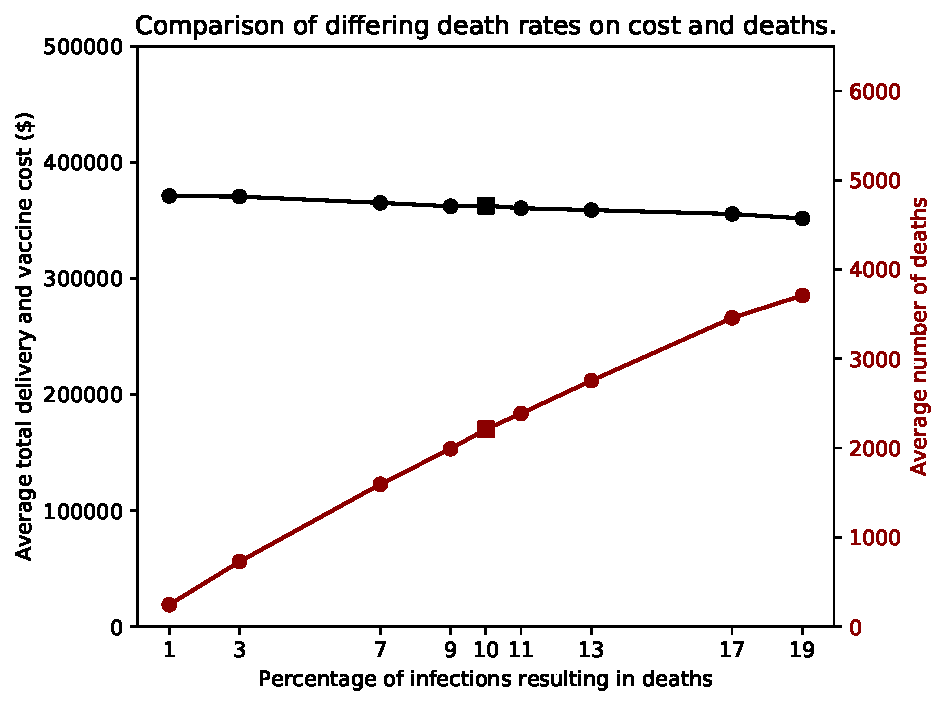
\includegraphics[width=0.48\textwidth, trim={0 0 0 0.67cm}, clip]{Figures/deathRate.pdf}
       \label{fig:deathRate}
     }
     \subfloat[Comparison of $R_{0}$ values.]{
       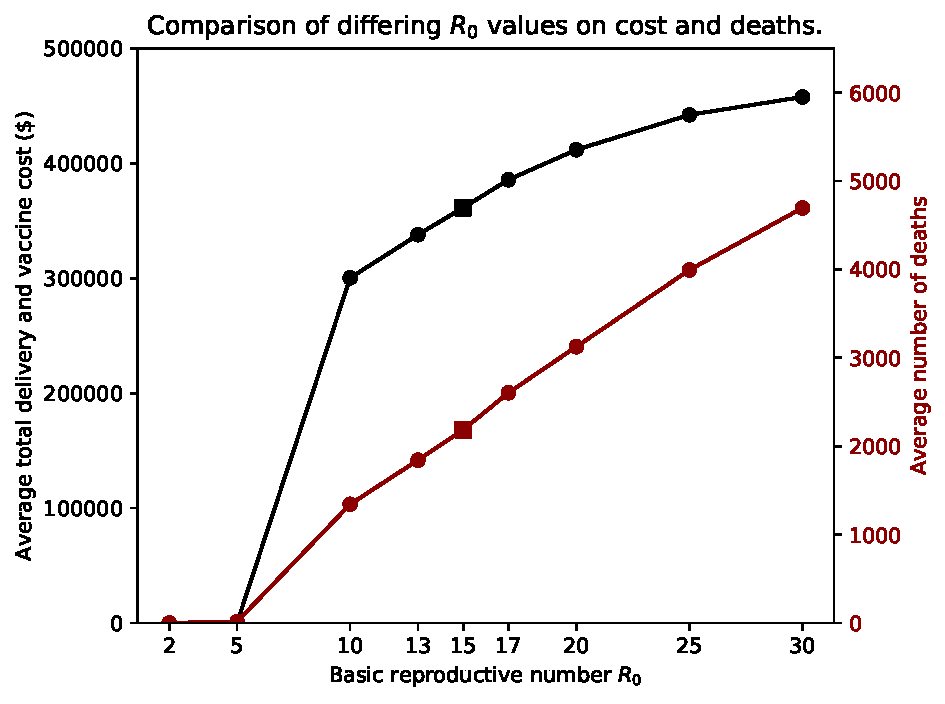
\includegraphics[width=0.48\textwidth, trim={0 0 0 0.67cm}, clip]{Figures/Rzero.pdf}
       \label{fig:Rzero}
     }
\caption{Effects of differing values for epidemic parameters on results.}
\end{figure}

The base values for the aforementioned parameters are discussed below:
\begin{itemize}
    \item $\sigma$ -- Reciprocal of the number of days in the E class between exposure and onset of symptoms. This is more intuitively understood as the proportion of people in the E class moving to the I class, daily. A base value of $\sigma = \frac{1}{10}$ is used, since infection usually follows 10 days after exposure \cite{who_2019}. The number of deaths and the average cost for differing durations of exposure are plotted in Figure \ref{fig:expDays}. As the number of days between exposure and onset of symptoms lengthens, the number of deaths decreases, while cost increases. This is because the epidemic would spread more slowly, allowing more vaccinations to be made before individuals become exposed -- resulting in the increased cost. Note that the cost appears to be more sensitive to changes in this parameter than the number of deaths, although even small increases in the number of deaths may be considered as significant, depending on the decision-maker.
    \item $\gamma$ -- Reciprocal of the number of days of symptoms and contagiousness in the I class. This value corresponds to the proportion of people in the I class moving to the R class daily, and a base value of $\gamma = \frac{1}{8}$ is used -- because infection usually lasts 8 days \cite{who_2019}. As may be seen in Figure \ref{fig:infDays}, if the duration of infection is longer, the number of deaths decreases. A longer duration results in a smaller value for $\gamma$, which in turn results in a smaller value of $\beta$, and the epidemic spreads more slowly.
    \item $\beta$ -- Proportion of the number of people in the S class moving to the E class daily. Note that $\beta = R_{0} \times \gamma$. The value of the basic reproductive number $R_{0}$ is cited much more often than the value of $\beta$, and thus, $\beta$ is calculated in terms of $R_{0}.$ In these simulations, $R_{0}$ is set to 15, meaning that an average of 15 total measles cases are caused by each infectious individual \cite{guerra2017basic}. Any increases in this $R_{0}$ value cause proportional increases in the number of deaths and cost; when the epidemic spreads faster, there is less time for vaccinations to occur. The model is very sensitive to changes in $R_{0}$. Note that for $R_{0}$ values of 5 and below, due to the rounding up and down of values and the small number of index cases, the epidemic usually dies out prematurely. Using continuous values instead of discrete would likely result in more accurate results for this parameter.
    \item $\mu$ -- Daily proportion of infected individuals that die. In literature the total proportion of deaths to infections is often given, so this total proportion is divided by the number of days of infection to get a daily value. Hence, $\mu = \texttt{Death Rate} \times \gamma$, with \texttt{Death Rate} set to 0.1 \cite{moss2007measles}. As expected, when \texttt{Death Rate} is increased, there is an almost exact proportional increase in the number of deaths, which can be seen in Figure \ref{fig:deathRate}. For obvious reasons, the number of deaths is more sensitive to changes in this parameter than the total cost, although cost decreases slightly as the death rate increases, due to the lower number of vaccinations which can occur when more people die.
    
    \begin{figure}[]
    \centering
    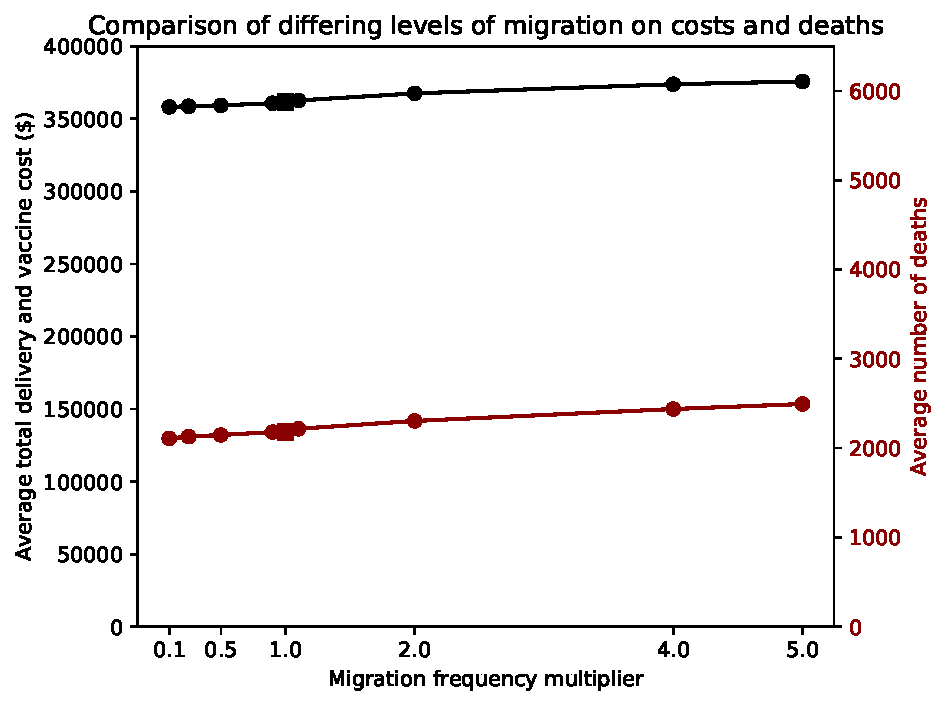
\includegraphics[width=0.5\textwidth, trim={0 0 0 0.67cm}, clip]{Figures/migrationFreq.pdf}
    \caption{Effect of differing levels of migration on results.}
    \label{fig:migrationFreq}
    \end{figure}
    
    \item $k_{m}$ -- Migration frequency multiplier. This is initially set to 1, so that there is no added migration to the basic gravity model of \S \ref{sec:meth_migration}. The amount of migration between locations in the network is directly proportional to this parameter value. The average results of the simulation are plotted in Figure \ref{fig:migrationFreq}, and it is evident in the figure that the model is not sensitive to changes in the amount of migration. As the amount of migration increases, the number of deaths also increase slightly -- because the epidemic spreads across the network faster. Having a high migration multiplier of 5 results in a 14.1\% increase in the number of deaths. Therefore, discouraging movement of individuals between locations during an outbreak can help to curb the spread of it, but is not very effective.
\end{itemize}

Additionally, the number of vaccinations which can occur in a network can be limited by the turnout of people for vaccinations. In urban areas where fixed-post teams are located, the turnout is assumed to be normally distributed with a mean of 900 and a variance of $\frac{900}{5}$. In rural areas, it is assumed to be normally distributed with a mean of 450 and a variance of $\frac{450}{5}$. These values correspond to those in \S \ref{meth:MeaslesCompa}. Varying each across a range of feasible values results in the points plotted in Figures \ref{fig:urbTnt} and \ref{fig:rurTnt}. In both cases, the sensitivity of the number of deaths to turnout is essentially negligible; the number of teams at a location is usually the limiting factor on vaccinations, rather than turnout. However, if turnout were to decrease even further towards the extreme value of zero, it is probable that the model results would become more sensitive to changes in turnout. If turnout was modelled such that it depended upon the progression of the epidemic, results would likely be more sensitive to changes in turnout. 

\begin{figure}[ht!]{\textwidth}
    \centering
     \subfloat[Effect of mean urban turnout on results.]{
       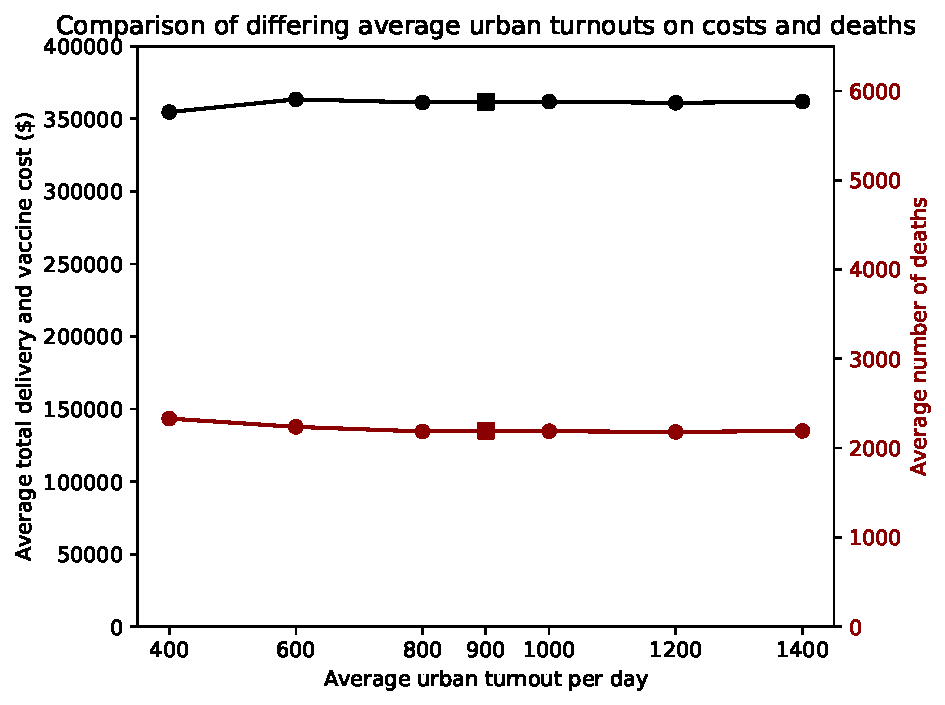
\includegraphics[width=0.48\textwidth, trim={0 0 0 0.67cm}, clip]{Figures/urbanTnt.pdf}
       \label{fig:urbTnt}
     }
     \subfloat[Effect of mean rural turnout on results.]{
       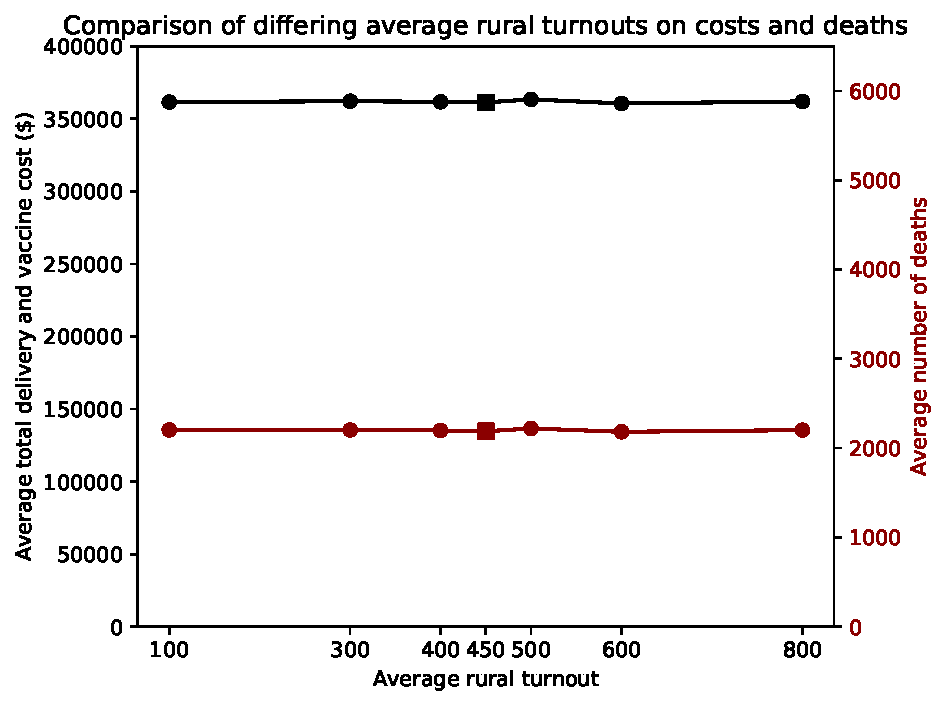
\includegraphics[width=0.48\textwidth, trim={0 0 0 0.67cm}, clip]{Figures/ruralTnt.pdf}
       \label{fig:rurTnt}
     }
\caption{Effect of differing turnout values for rural and urban areas on costs and deaths.}
\end{figure}

\subsubsection{Vaccine-related parameters}
The success rate of the measles vaccine depends on whether the individual receiving the vaccine has been exposed to the measles virus, and whether they have received a dose of the vaccine before. It is assumed that all individuals in the S class have never received a dose of any measles vaccine.
An estimated 2-5\% of first-dose measles vaccinations are unsuccessful \cite{cdc_pinkbook_2018}, so the probability of a vaccinated individual moving from state S to R -- the vaccine success rate $\lambda_{S}$ -- can be reasonably set to $\lambda_{S} = 95\%$. Values ranging between 80\% and 100\% for this success rate were tested, with results plotted in Figure \ref{fig:vaccEfficacy}. It is clear that if the vaccine is more successful or less successful, the only notable difference in results is a slight change in cost, and so the model output is not very sensitive to this parameter.

\begin{figure}[ht!]{\textwidth}
    \centering
     \subfloat[Effect of changes in vaccine efficacy $\lambda_{S}$.]{
       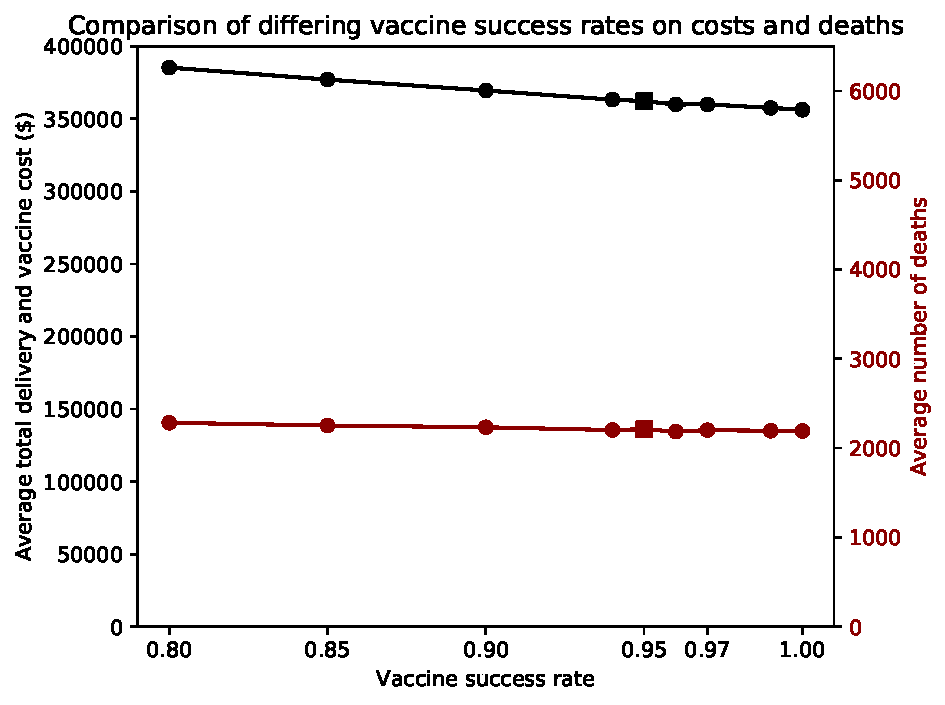
\includegraphics[width=0.48\textwidth, trim={0 0 0 0.67cm}, clip]{Figures/vaccSuccessRate.pdf}
       \label{fig:vaccEfficacy}
     } 
     \subfloat[Effect of changes in prophylaxis efficacy $\lambda_{E}$ .]{
       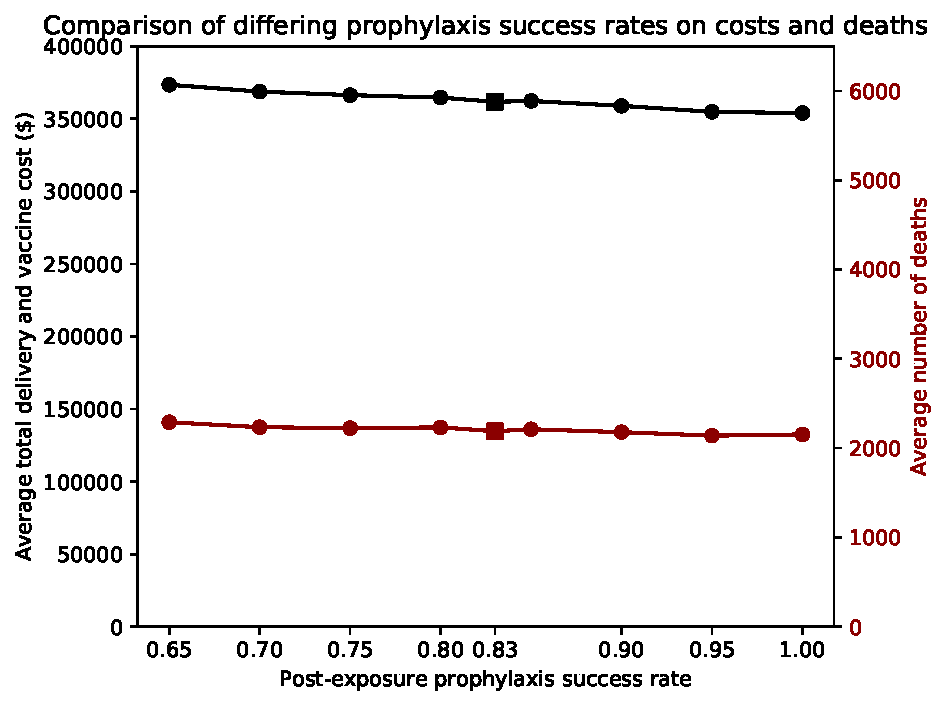
\includegraphics[width=0.48\textwidth, trim={0 0 0 0.67cm}, clip]{Figures/prophEffectiveness.pdf}
       \label{fig:prophEfficacy}
     }
     \vspace{2pt}
     \subfloat[Effect of differing vaccine potency duration values.]{
       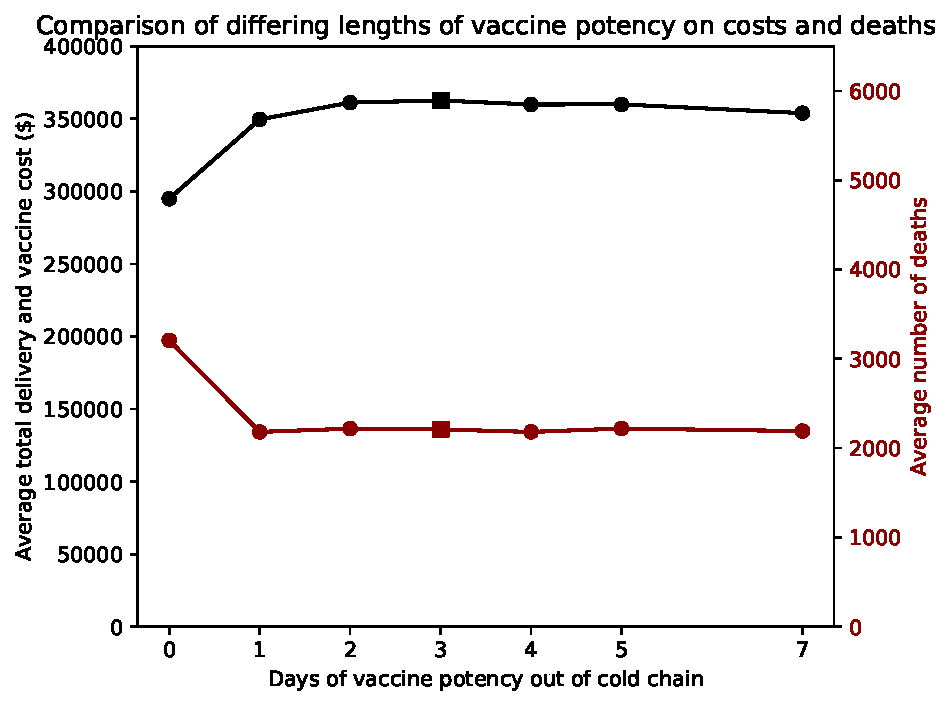
\includegraphics[width=0.48\textwidth, trim={0 0 0 0.67cm}, clip]{Figures/monoDaysPotency.pdf}
       \label{fig:monoDosePotency}
     }
\caption{Sensitivity of vaccine-related parameters.}
\end{figure}

If the individual has only been exposed to the virus for less than 72 hours, they can be given post-exposure prophylaxis. In a 2006 study in Australia, the effectiveness of this prophylaxis for measles cases was found to be 83\% \cite{csiro_2009}. Thus the prophylaxis success rate can be set to $\lambda_{E} = 83\%$. It is thus assumed that 83\% of individuals given prophylaxis are moved directly from the E to the V class, and do not become infectious. As is seen in Figure \ref{fig:prophEfficacy}, values ranging between 65\% and 100\% were tested, with only a slight decrease in deaths and cost as the success rate rises, so the model output is not very sensitive to this parameter.

The measles vaccine can remain at the required potency level outside of the cold chain for 3 days \cite{msf_ectc_2018}. Were this value to change, or even reduce to only a single day, there would be essentially no change in the number of deaths. Figure \ref{fig:monoDosePotency} shows the average number of deaths and total cost for different lengths of potency. There is only an increase in the number of deaths if the vaccine needs to be used on the same day as it is delivered -- and even then, the number of deaths is half of what it would be if there was no intervention. Therefore, transporting the measles vaccine outside of the cold chain is feasible and can considerably reduce cost when compared to the existing cold chain.

\subsubsection{Delivery parameters}
The final set of parameters to be tested for sensitivity are those affecting the delivery network. For the sensitivity analysis pertaining to UAV deliveries, the vaccine allocation strategy $I$ and team allocation strategy $N$ were used, as in the case of vehicle deliveries.

\label{sec:res_del_params}
\begin{itemize}
    \item \textit{The average UAV speed, in kilometres per hour.} An initial value of 100 km/h is used \cite{czerwonka_2018,service_contract_2018, zipline_impact}, and the speed is varied between 20 km/h and 180 km/h to test the impact different speeds have on results. As may be seen in Figure \ref{fig:res_UAVspeed}, results are insensitive to increases in average UAV speed, but sensitive to decreases in average speed below 80km/h. Any slower, and deaths begin to rise as the average speed decreases; because slower UAVs result in teams' requirement for vaccines not being met quickly enough. Therefore, fixed-wing UAVs would be better than the generally slower quadcopters for a network such as this.
    \item \textit{The number of vaccine doses that one UAV can deliver per flight.} A base value of 60 is used, as per the calculations in \S \ref{sec:dro_dels}. Figure \ref{fig:res_UAVcap} shows that as long as UAVs can carry over 30 vaccines, there is no reduction in the average number of deaths. If a UAV could only carry 10 vaccines per flight, the average number of deaths would rise by just under 200. So, with only two UAVs, the UAV-only delivery network is almost able to completely fulfill vaccine demand.
    \item \textit{The number of vaccine doses that vehicles can deliver per route.} Recall that vehicle deliveries are modelled such that routes having any rural areas in them are delivered to by a smaller, secondary vehicle, while all other routes are visited by a primary vehicle. There is initially assumed to be one of each type in the vehicle-only network. Figures \ref{fig:res_primVehCap} and \ref{fig:res_secVehCap} show the results of 500 simulations each for a range of vehicle capacities. Clearly, the vehicle network is able to completely meet vaccine demand, no matter what the capacity of each vehicle is -- provided the capacity is within the tested range.
    \item \textit{The combined network cutoff time.} The combined delivery network, using 1 UAV and 1 vehicle, allows UAVs to deliver to areas that a vehicle would take too long to deliver to. Initially, the maximum allowed vehicle route time is 3 hours. Clearly, other thresholds than 3 hours could also be used with similar success; as can be seen in Figure \ref{fig:res_comboCutoff}, the model output is not very sensitive to changes in this threshold.
\end{itemize}

\begin{figure}[ht!]{\textwidth}
\centering
\subfloat[Effect of differing average UAV speeds on results.]{
   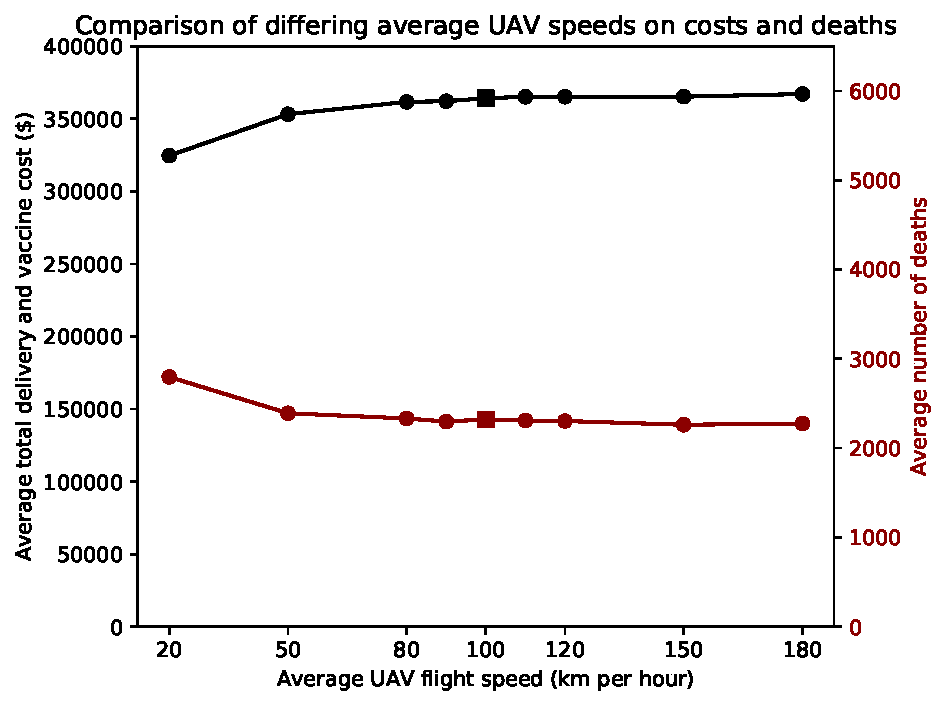
\includegraphics[width=0.47\textwidth, trim={0 0 0 0.67cm}, clip]{Figures/UAVspeed.pdf}
   \label{fig:res_UAVspeed}
 } \hspace{1}
 \subfloat[Effect of differing UAV vaccine capacities on results.]{
   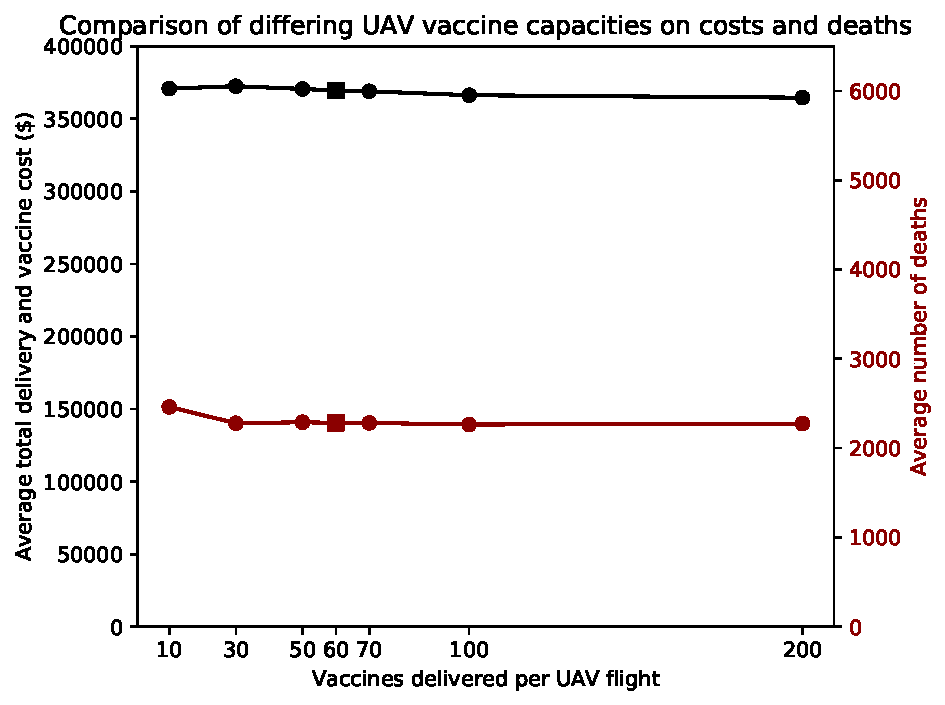
\includegraphics[width=0.47\textwidth, trim={0 0 0 0.67cm}, clip]{Figures/UAVcapacity.pdf}
   \label{fig:res_UAVcap}
 } \vspace{1}
\subfloat[Effect of differing primary vehicle    capacities on results.]{
   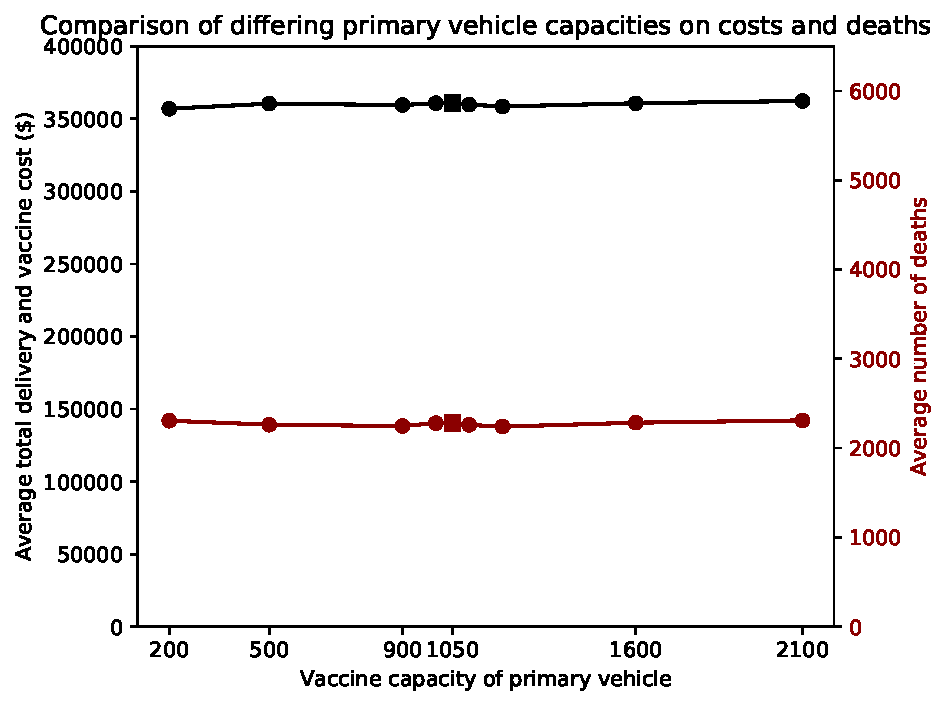
\includegraphics[width=0.47\textwidth, trim={0 0 0 0.67cm}, clip]{Figures/primVehCap.pdf}
   \label{fig:res_primVehCap}
} \hspace{1}
\subfloat[Effect of differing secondary vehicle capacities on results.]{
   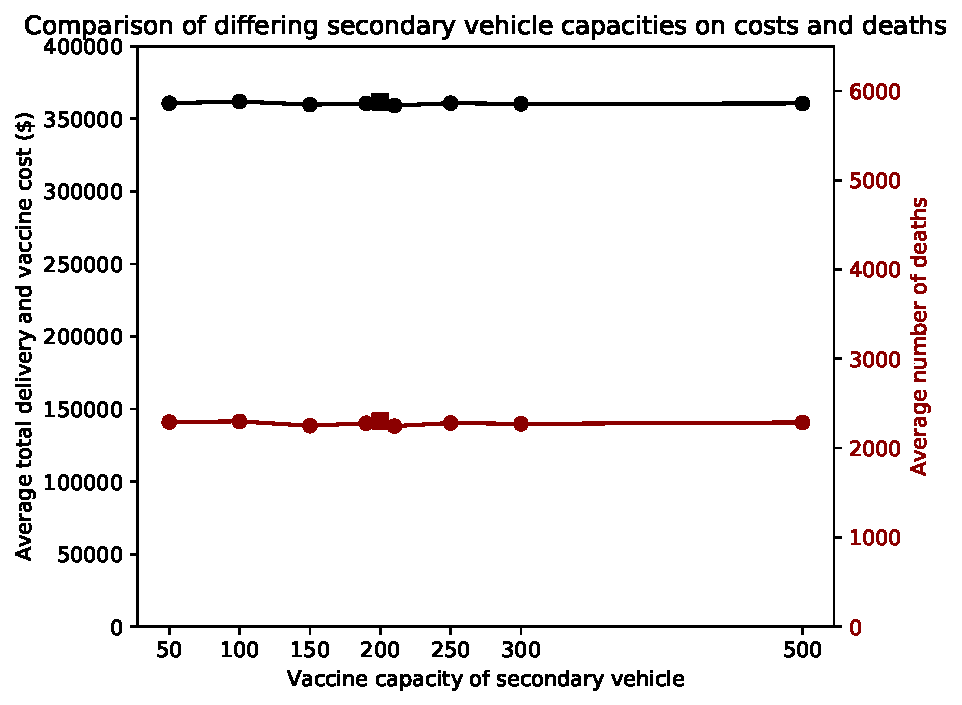
\includegraphics[width=0.47\textwidth, trim={0 0 0 0.67cm}, clip]{Figures/secVehCap.pdf}
   \label{fig:res_secVehCap}
 } \vspace{1}
\subfloat[Effect of cutoff values for combined delivery network on results.]{
   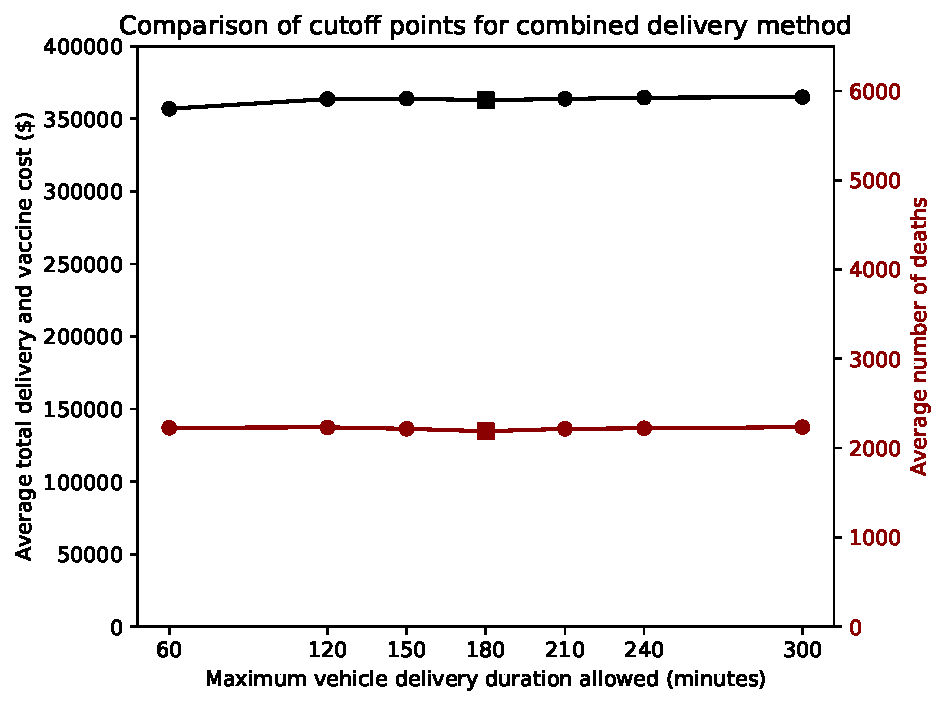
\includegraphics[width=0.47\textwidth, trim={0 0 0 0.67cm}, clip]{Figures/combinedCutoffMins.pdf}
   \label{fig:res_comboCutoff}
 }
\label{fig:deliverySensitivity}
\caption{Comparison of values for delivery-related parameters.}
\end{figure}

\section{Scenario Tests}
\label{sec:res_scenTests}
The factors in an epidemic intervention that can be controlled by decision makers include decisions about who to vaccinate, teams, and intervention timing.

\subsection{Vaccination targeting}
\begin{table}[ht!]
\centering
\begin{tabular}{|c|c|c|}
\hline
\textbf{Metric}  & \multicolumn{1}{c|}{\textbf{Targeted Vaccination}} & \textbf{Untargeted Vaccination} \\ \hline
Deaths           & 2\,212                                             & 4\,218                          \\ \cline{1-1}
Cost             & \$362\,523                                         & \$596\,345                      \\ \cline{1-1}
Vaccinations     & 121\,691                                            & 187\,656                        \\ \cline{1-1}
Vaccines Expired & 4\,969                                             & 17\,239                         \\ \hline
\end{tabular}
\caption{Comparison of targeted vaccination with untargeted vaccination, with values obtained from 500 simulations using each policy.}
\label{tab:res_targetedVacc}
\end{table}

Recall that vaccination can either be targeted (where only those individuals without a previous history of vaccination are vaccinated) or untargeted (where everybody is vaccinated, regardless of vaccination history). Interventions with targeted vaccination are generally more effective since vaccines are only given to those who actually need them, but a drawback of this policy is that documentation about vaccination history may not be available, and that it is usually easier in outbreak response to vaccinate non-selectively. Table \ref{tab:res_targetedVacc} contains the average results of a comparison between the two policies, with each simulated 500 times. Standard deviation is low in both cases. As is clear in the table, there are nearly double the amount of deaths in the case of untargeted vaccination, since a lot of vaccines are `wasted' on already-immune individuals. Without these wasted vaccines, the average cost of targeted vaccination is 39.2\% less than untargeted vaccination. Thus, it is clear that targeted vaccination is significantly better in epidemic response, and dramatically reduces costs and deaths.


\subsection{Team-related parameters}
Vaccination teams are perhaps the most important part of an epidemic response. It is essential to send teams to locations such that the right people are vaccinated on time, in order to curb the epidemic. Three team-related factors can be adjusted in the simulation model:

\begin{itemize}
    \item \textit{The number of (on-duty) vaccination teams in the entire network.} This is set to a constant value of 15 teams initially. The number of teams in the network varies significantly according to the severity of an outbreak, so there is no established, constant number of teams. In a 2016 cholera outbreak response in Zambia, there was a maximum of 17 teams used across 10 locations \cite{poncin2018implementation}, a case similar to the considered network, so 15 is a good general estimate. This is simulated for values ranging from 5 to 25, the results of which can be seen in Figure \ref{fig:vaccTeams}. The figure has two axes; black for average total vaccination and delivery cost incurred, and red for the average number of deaths. Each point is the average result of 500 simulations with that point's number of teams, and the point for the initial value of the number of teams is marked with a square instead of a circle. It is clear that the number of teams in the network has a large impact on the number of deaths and the cost, although this impact decreases as more teams are added. Note that the cost plotted is only the delivery and vaccine cost, and does not include any costs for teams or volunteers. Therefore, since having more teams certainly would incur additional costs, a tradeoff needs to be made, with the number of teams used limited.
    
    \begin{figure}[ht!]{\textwidth}
    \centering
     \subfloat[Comparison of differing numbers of teams.]{
       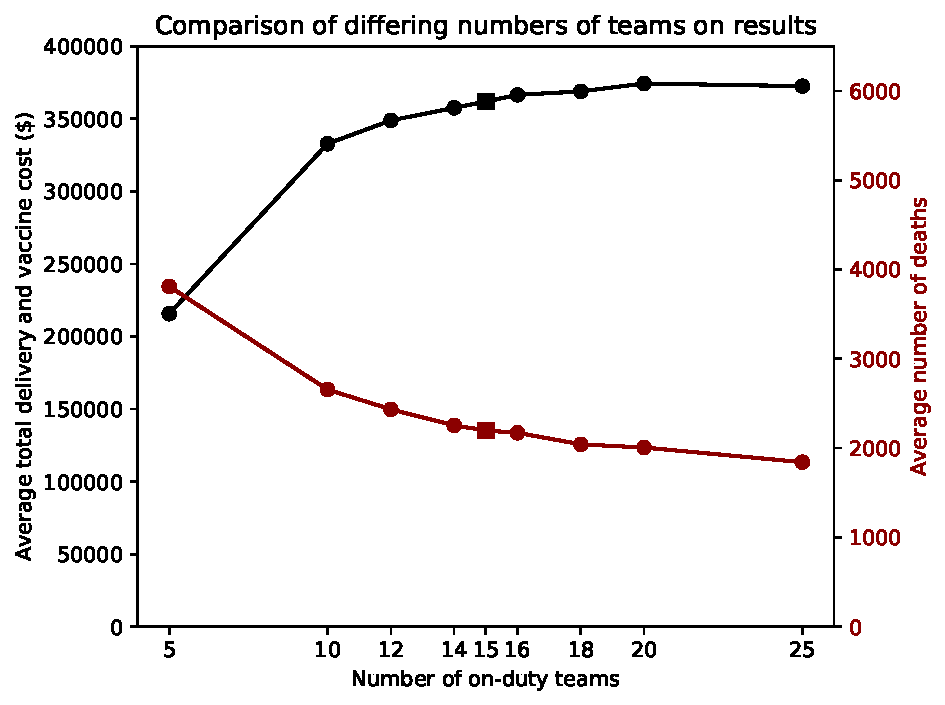
\includegraphics[width=0.48\textwidth, trim={0 0 0 0.67cm}, clip]{Figures/NumberTeams.pdf}
       \label{fig:vaccTeams}
     }
     \subfloat[Comparison of differing daily working minutes.]{
       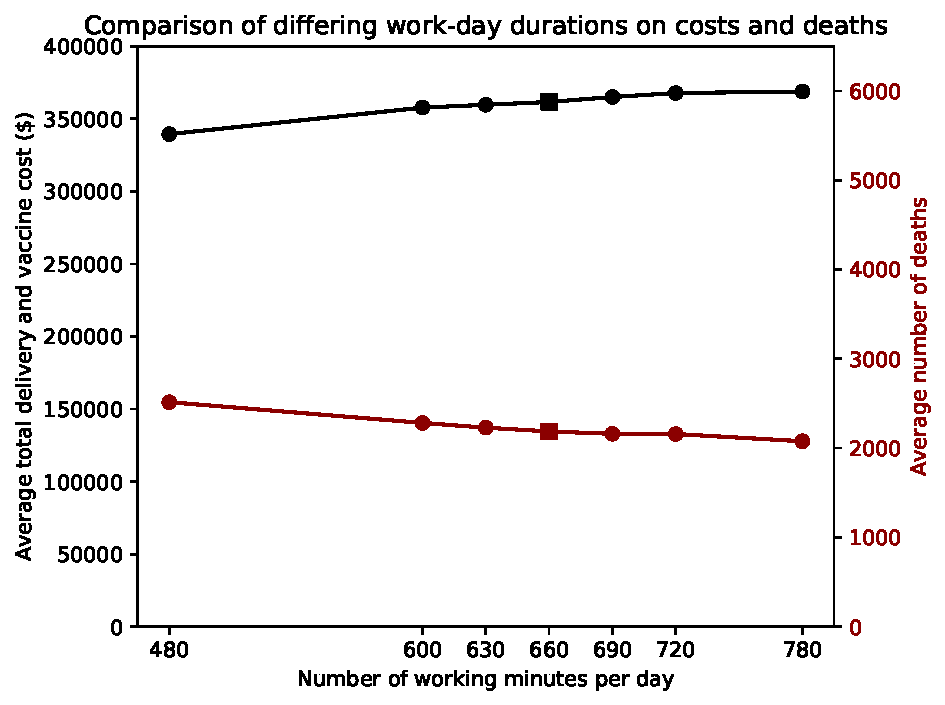
\includegraphics[width=0.48\textwidth, trim={0 0 0 0.67cm}, clip]{Figures/NumberMinsday.pdf}
       \label{fig:vaccMins}
     }
     \vspace{2}
     \subfloat[Comparison of differing weekly working days.]{
       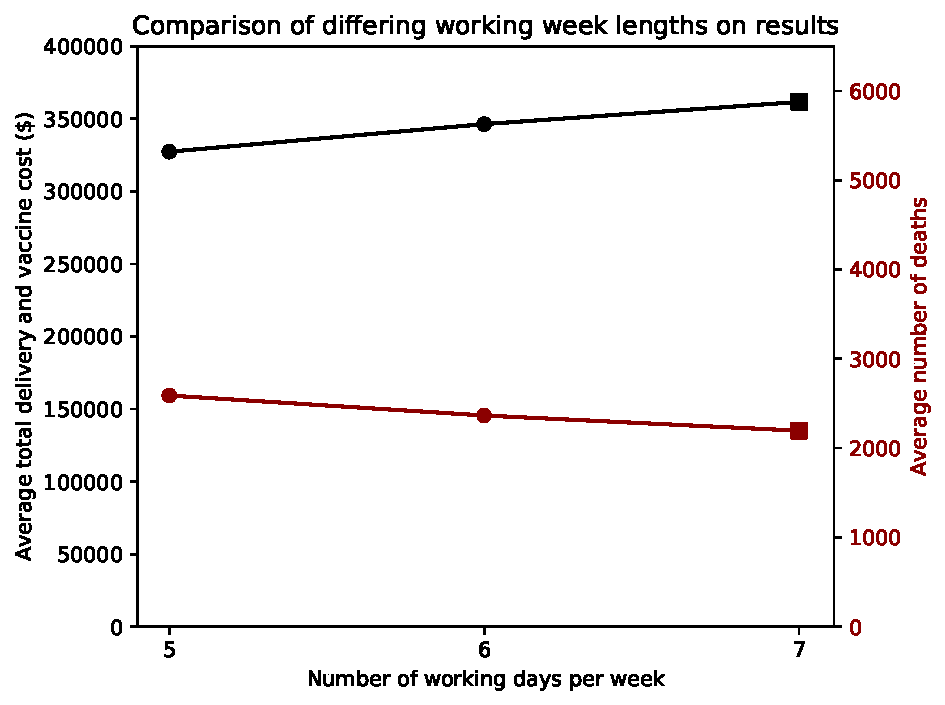
\includegraphics[width=0.48\textwidth, trim={0 0 0 0.67cm}, clip]{Figures/NumberDaysweek.pdf}
       \label{fig:teamWorkDays}
     }
    \caption{Effects of differing values for team-related parameters on cost and deaths.}
    \end{figure}
    
    \item \textit{The number of working minutes for vaccination teams and deliveries per day.} This value is initially set to 660, corresponding to an 11 hour working day \cite{poncin2018implementation}, but is varied between 480 and 780 (8 hours and 13 hours, respectively), producing the results depicted in Figure \ref{fig:vaccMins}. There is a visible impact of the number of minutes worked per day on the number of total deaths and cost; as daily minutes worked increases, the number of deaths decreases. In fact, for each minute above 480 worked each day, the number of deaths reduces by an average of 1.46, while the cost increases by \$97.86. Therefore, working for as long as possible each day is essential, particularly at the crucial beginning stages of the intervention.
    \item \textit{The number of working days for vaccination teams and deliveries per week.} Initially, a full working week of 7 days is assumed. This can be accomplished by having teams working on shifts, so that some teams are able to take time off while others continue to vaccinate. There is simply assumed to be a constant number of 15 teams on duty, 7 days a week. That way, any number of teams can be off duty, as long as 15 are working. To account for 6-day or 5-day work weeks, where on the day(s) off neither deliveries nor vaccinations occur, days are randomly chosen to be taken off with a probability of $\frac{6}{7}$, or $\frac{5}{7}$, respectively. As can be seen in Figure \ref{fig:teamWorkDays}, there is a significant difference in the number of deaths if fewer than 7 days are worked per week. Working 6 days a week instead of 7 results in an average of 170 more deaths, and working 5 days instead of 7 causes an average of 394 more.
    
    To test whether overlapping shifts are significantly better than all teams having a shared day off, two simulations are repeated 500 times each. The first is an intervention with 14 teams, 6 days per week. The second is one with 12 teams, working 7 days per week. Note the total hours worked is the same in both cases, yet the case with 12 teams in overlapping shifts reduces average deaths by nearly 20. The results of this comparison are shown in Table \ref{tab:shiftsVs6days}. Performing a hypothesis test to compare these two deaths means for equality concludes that the null hypothesis (that they are equal) is rejected, with a p-value of less than 0.0001 -- the 95\% confidence interval of the difference between the two is \{-20.9111, -16.2889\}. Thus, overlapping shifts are significantly better than shared days off, in the simulations conducted.
    
    \begin{table}[ht!]
    \centering
    \resizebox{\textwidth}{!}{%
    \begin{tabular}{|cc|ccc|}
    \hline
    \multicolumn{1}{|c|}{Number of teams on duty} & Work days per week & \multicolumn{1}{c|}{Average deaths} & \multicolumn{1}{c|}{Average cost} & Average vaccines spoiled \\ \hline
    14 & 6 & 2453.3 & 340\,512 & 6807.8 \\
    12 & 7 & 2434.7 & 348\,866 & 6474.7 \\ \hline
    \end{tabular}%
    }
    \caption{Comparison of overlapping shifts against all teams having a common day off}
    \label{tab:shiftsVs6days}
    \end{table}
    
    \item \textit{The number of vaccinations that teams can perform daily.} This value is initially set to 450 vaccinations per day for fixed-post teams, and to 250 for mobile teams, as in \S \ref{meth:MeaslesCompa}. These values are each ranged between 100 and 800, and 50 and 450, respectively; with results plotted in Figures \ref{fig:fixedVaccAbility} and \ref{fig:mobileVaccAbility}. It is obvious in the figures that if each fixed-post team could vaccinate more people daily, the intervention would be able to reduce the average total deaths considerably. The same does not hold for mobile teams; there is hardly any impact of changes in teams' abilities to vaccinate, although this is largely a result of the considered network being mostly urban areas (so, using more fixed teams).
    
    \begin{figure}[ht!]{\textwidth}
    \centering
     \subfloat[Comparison of fixed-post teams' daily ability to vaccinate.]{
       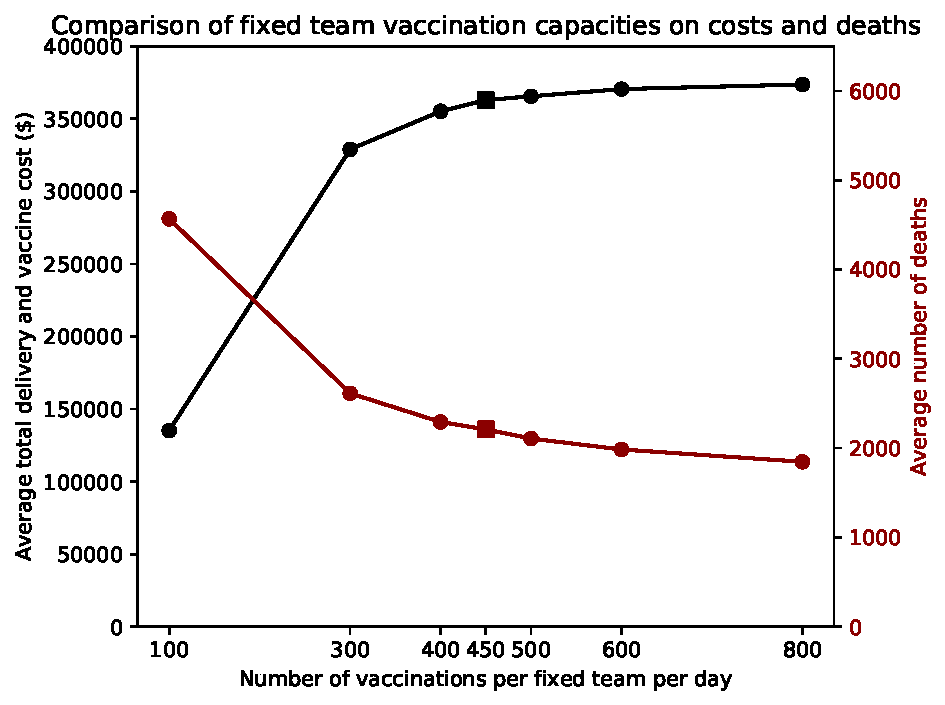
\includegraphics[width=0.48\textwidth, trim={0 0 0 0.67cm}, clip]{Figures/fixedVaccAbility.pdf}
       \label{fig:fixedVaccAbility}
     }
     \vspace{2}
     \subfloat[Comparison of mobile teams' daily ability to vaccinate.]{
       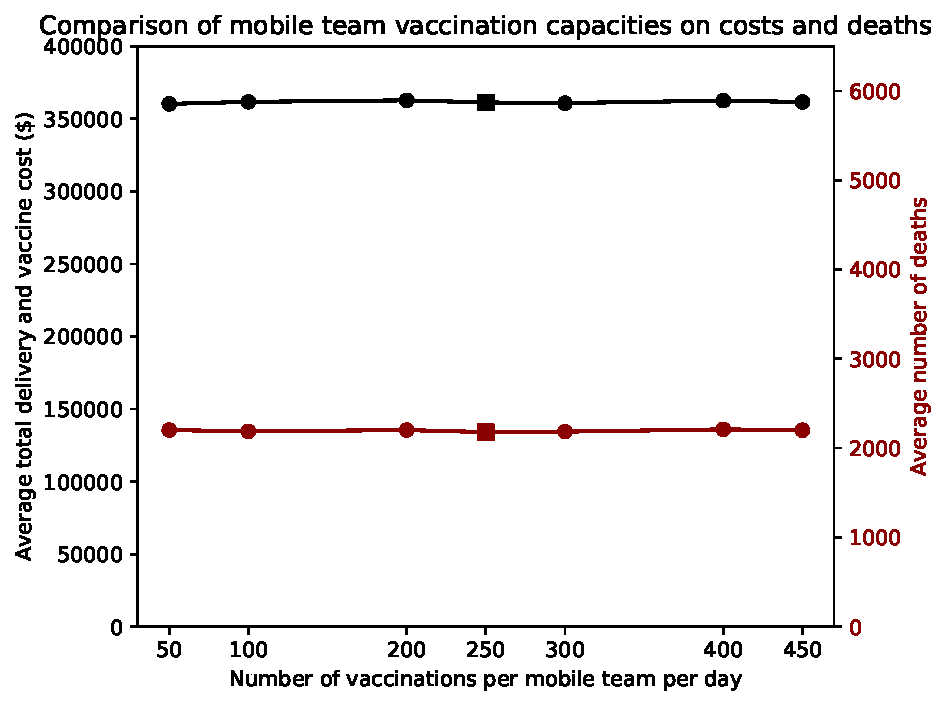
\includegraphics[width=0.48\textwidth, trim={0 0 0 0.67cm}, clip]{Figures/mobileVaccAbility.pdf}
       \label{fig:mobileVaccAbility}
     }
    \caption{Comparing results of different team abilities for vaccinations per day.}
    \end{figure}
    
\end{itemize}

\subsection{Intervention timing parameters}
The final set of parameters that decision makers can vary involve aspects of intervention timing. It is well known that the earlier an intervention begins, the more effective it will be, and this is confirmed by the results found, along with two other important results. The following parameters are tested for differing values:

\begin{itemize}
    \item \textit{The proportion of the population at any location to be infected before an epidemic is declared.} A simple method of declaring the epidemic is used for this project; once the ratio of infectious individuals to the population in any area exceeds a certain threshold (this parameter value), the epidemic is declared, and preparations begin for the intervention to start. An initial proportion of 0.5\% is used. This method is intuitive, because the higher the proportion of infections to population, the more noticeable the infections will be to local health workers, and so the epidemic would be declared. Different values of this threshold are plotted as percentages in Figure \ref{fig:intThres}. Clearly, the simulation output is very sensitive to changes in this threshold. The longer it takes for an epidemic to be declared and for vaccinations to begin, the more deaths. Practically, this detection threshold could be improved by educating local health workers to recognise measles cases better, and to understand the risks of measles. It is difficult to estimate what an accurate value for this threshold would be. Comparing real-life epidemic detection methods is a useful topic for future research.
    
    \begin{figure}[ht!]{\textwidth}
    \centering
     \subfloat[Comparison of epidemic declaration thresholds.]{
       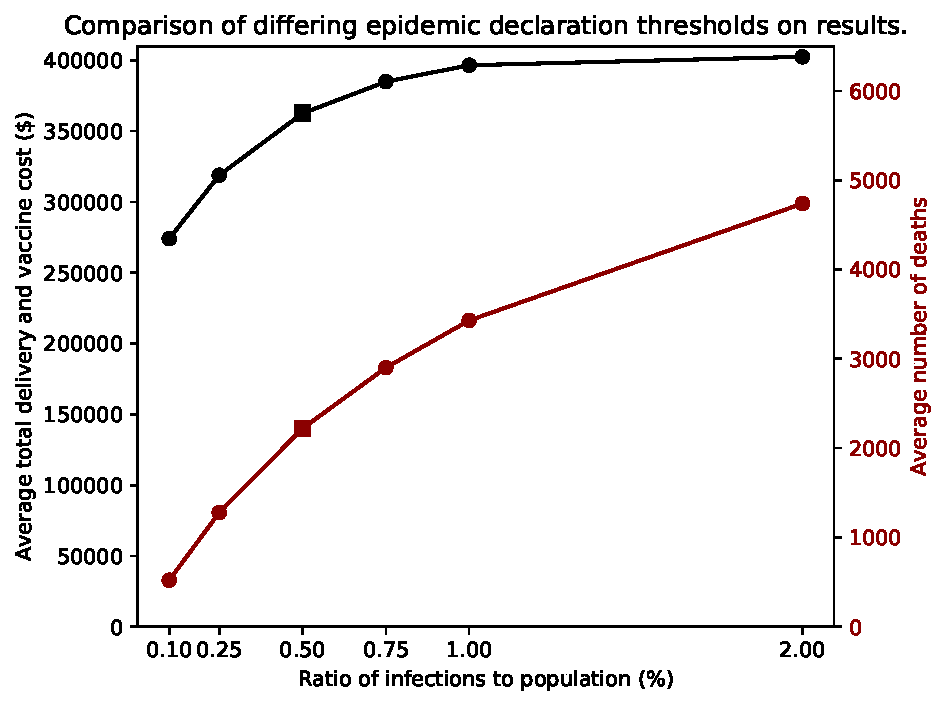
\includegraphics[width=0.48\textwidth, trim={0 0 0 0.67cm}, clip]{Figures/IntThreshold.pdf}
       \label{fig:intThres}
     }
     \subfloat[Comparison of differing intervention delays.]{
       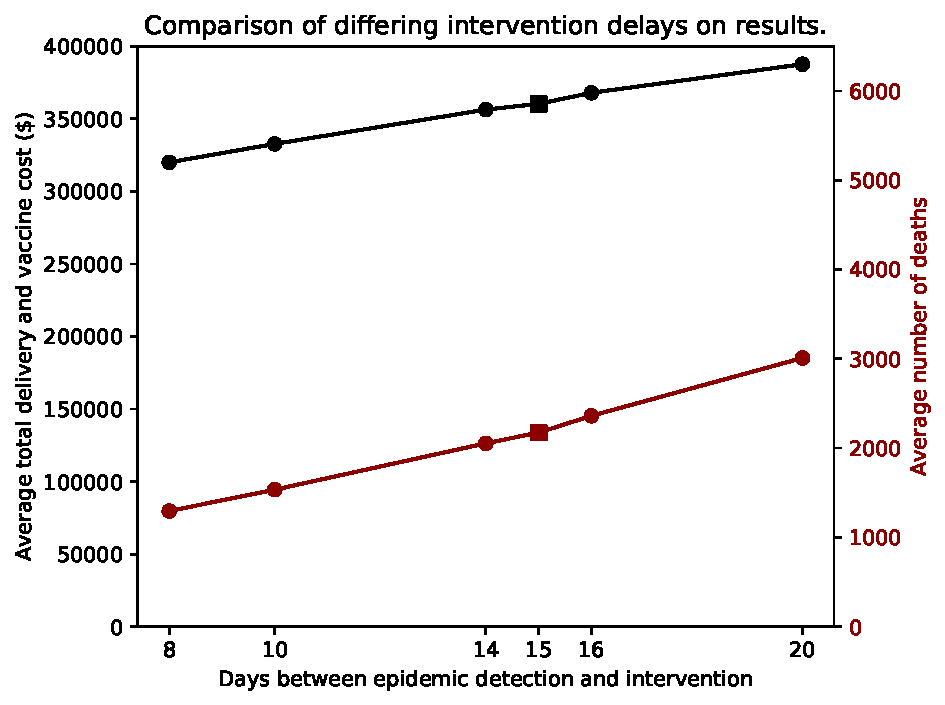
\includegraphics[width=0.48\textwidth, trim={0 0 0 0.67cm}, clip]{Figures/IntLeadTime.pdf}
       \label{fig:intLeadTime}
     }
     \vspace{2pt}
     \subfloat[Comparison of differing intervention lengths.]{
       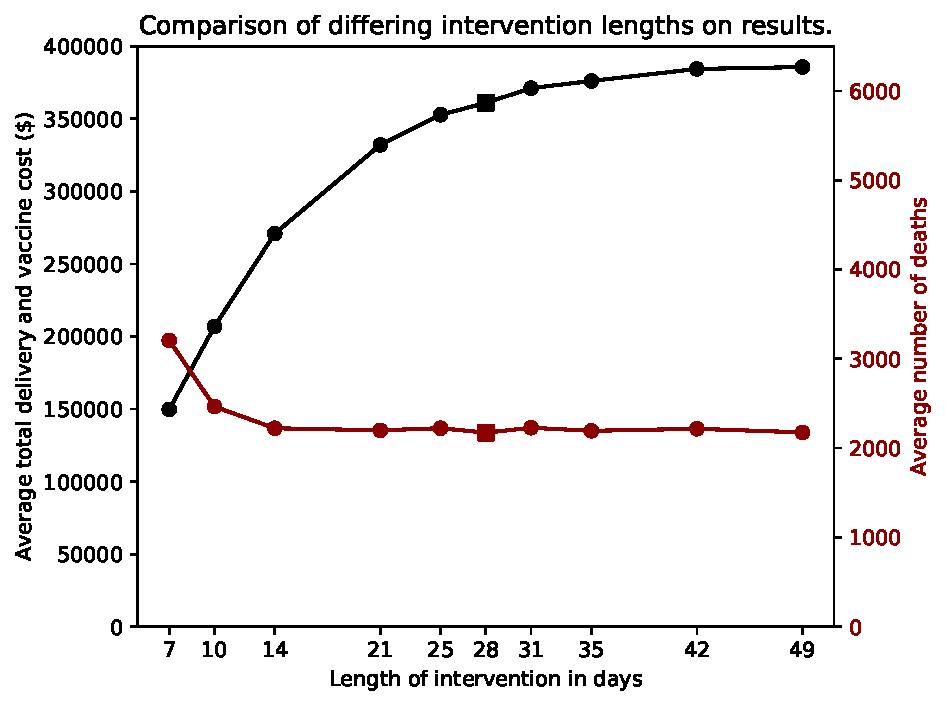
\includegraphics[width=0.48\textwidth, trim={0 0 0 0.67cm}, clip]{Figures/IntLength.pdf}
       \label{fig:intLength}
     }
    \caption{Effects of differing values for team-related parameters on cost and deaths.}
    \end{figure}
    
    \item \textit{The number of days after the epidemic has been detected, until intervention begins.} MSF states that,
    "emergency vaccination campaign preparation should not take more than two weeks," and that, "ideally, emergency vaccination activities can be set up in 8 to 10 days, 15 days maximum" 
    \cite{danet_fermon_2013}. The delay before intervention is a much-discussed topic in epidemic response, and although it is well known that the response needs to be as prompt as possible, it is often difficult to set up the delivery network and get teams on the ground more quickly. Were a UAV network to be used in the future, it would need to be set up from scratch within 8-10 days, ideally. As can be seen in Figure \ref{fig:intLeadTime}, the number of deaths increases in a linear fashion as the delay increases. For each extra day of delay above 8, there is a simulated average of 143 more deaths.
    
    \item \textit{Length of intervention in days.} The length of an intervention depends largely on the severity of an epidemic, and so, the results depicted in Figure \ref{fig:intLength} apply specifically to the case of this measles outbreak. An initial length of 28 days is used so that strategies can be compared for long enough. A useful result shown in the figure is that although vaccinations continue after day 14 (and costs continue to rise), the number of deaths does not decrease. This is likely because nearly all of the susceptible individuals in the network can be vaccinated within 14 days with a good team allocation. Even after 7 days of intervention, the average total number of deaths (3206) is less than half of what it would've been without an intervention (6504).
\end{itemize}